\documentclass[conference]{IEEEtran}

\usepackage{cite}


\ifCLASSINFOpdf
  \usepackage[pdftex]{graphicx}

  \graphicspath{{../pdf/}{../jpeg/}}

  \DeclareGraphicsExtensions{.pdf,.jpeg,.png}
\else

\fi

\usepackage{caption}
\usepackage{subcaption}

\usepackage{amsmath}
\usepackage{multirow}
\usepackage{multicol}

\usepackage{algorithmic}

\usepackage{array}
\usepackage{color}

\hyphenation{op-tical net-works semi-conduc-tor}


\begin{document}

\title{On-Chip Output Stage Design for a  Continuous Class F Power Amplifier}

\author{\IEEEauthorblockN{Anil Kumar Kumaran\IEEEauthorrefmark{1},
M. D'Avino\IEEEauthorrefmark{2},
Leo C.N. de Vreede\IEEEauthorrefmark{1}, and 
Morteza S. Alavi 
\IEEEauthorrefmark{1}} 
\IEEEauthorblockA{\IEEEauthorrefmark{1} Electronic Circuits and Architecture (ELCA) Research Group, Delft University of Technology \\
	\IEEEauthorblockA{\IEEEauthorrefmark{2} Catena B.V., Delft, The Netherlands} Email: a.k.kumaran@tudelft.nl}}

\maketitle

\begin{abstract}
Continuous Class F (CCF) power amplifiers (PAs) overcome Class F PA's disadvantage of narrow bandwidth by eliminating short-circuit requirements at the $2^{nd}$ harmonic. At the same time, CCF maintains a peak efficiency of \textit{90.7\%}, which is higher than the traditional Class A and B peak efficiency. This paper explains the equations governing the CCF mode of operation and then illustrates the step by step procedure to design  four different output networks for CCF using lossless lumped components for a \textit{2.1--2.7 GHz} band.
The design comprising a second harmonic trap and no RF choke is chosen due to its flatter real part impedance and smaller reactive part at the fundamental, and  the least number of on-chip lumped components.
\color{blue}The chosen design is implemented in TSMC 40 nm and has a passive efficiency of \textit{52\%}.\color{black} 
\end{abstract}

\vspace{1mm}
% keywords
\begin{IEEEkeywords}
Continuous class F (CCF), Output matching network, Power amplifier (PA), Harmonic termination, Differential mode analysis, Common mode analysis. 
\end{IEEEkeywords}

%\vspace{-0.1in}

\ifCLASSOPTIONpeerreview
\begin{center} \bfseries EDICS Category: 3-BBND \end{center}
\fi

\IEEEpeerreviewmaketitle

\section{Introduction}
Today, there is an increased demand for high-speed and low-cost transmissions in 4/5G and wireless connectivity networks. A CMOS-based transmitter (TX) is a viable architecture to address these requirements as it facilitates the implementation of System-on-Chip (SoC) solution at a low cost. However, the TX power amplifier (PA) is the most challenging blocks in making CMOS SoC, because it should offer high-efficiency while meeting the stringent spectral mask  and in-band linearity requirements of wireless systems even at backed-off power levels. Currently, most of TX architectures employ linear class A/B PAs. Nevertheless, their ideal  peak efficiencies are only \textit{50}/\textit{78\%}, respectively, due to a large overlap between the drain voltage/current waveforms (Fig.\ref{fig:wave_VI}a/b).

On the other hand, class F PAs ideally achieve peak efficiency of \textit{100\%} by utilizing harmonic-frequency resonators to short-circuit at even harmonics and open-circuit at odd harmonics leading to non-overlap drain voltage/current waveforms (Fig. \ref{fig:ICF_wave_VI}). Nevertheless, in reality, controlling all harmonics is challenging and increases the network complexity and component losses, degrading its passive efficiency. Therefore, practical implementation of class F employs up to $3^{rd}$ harmonic impedance terminations and achieves a peak efficiency of \textit{90.7\%} due to increasing the overlap region between the drain voltage and current compared to the ideal class F (Fig. \ref{fig:ICF_wave_VI}) \cite{Raab_max_eff}.
\begin{figure}[!t]
\centering
\captionsetup{font=footnotesize}
\begin{subfigure}{0.24\textwidth}
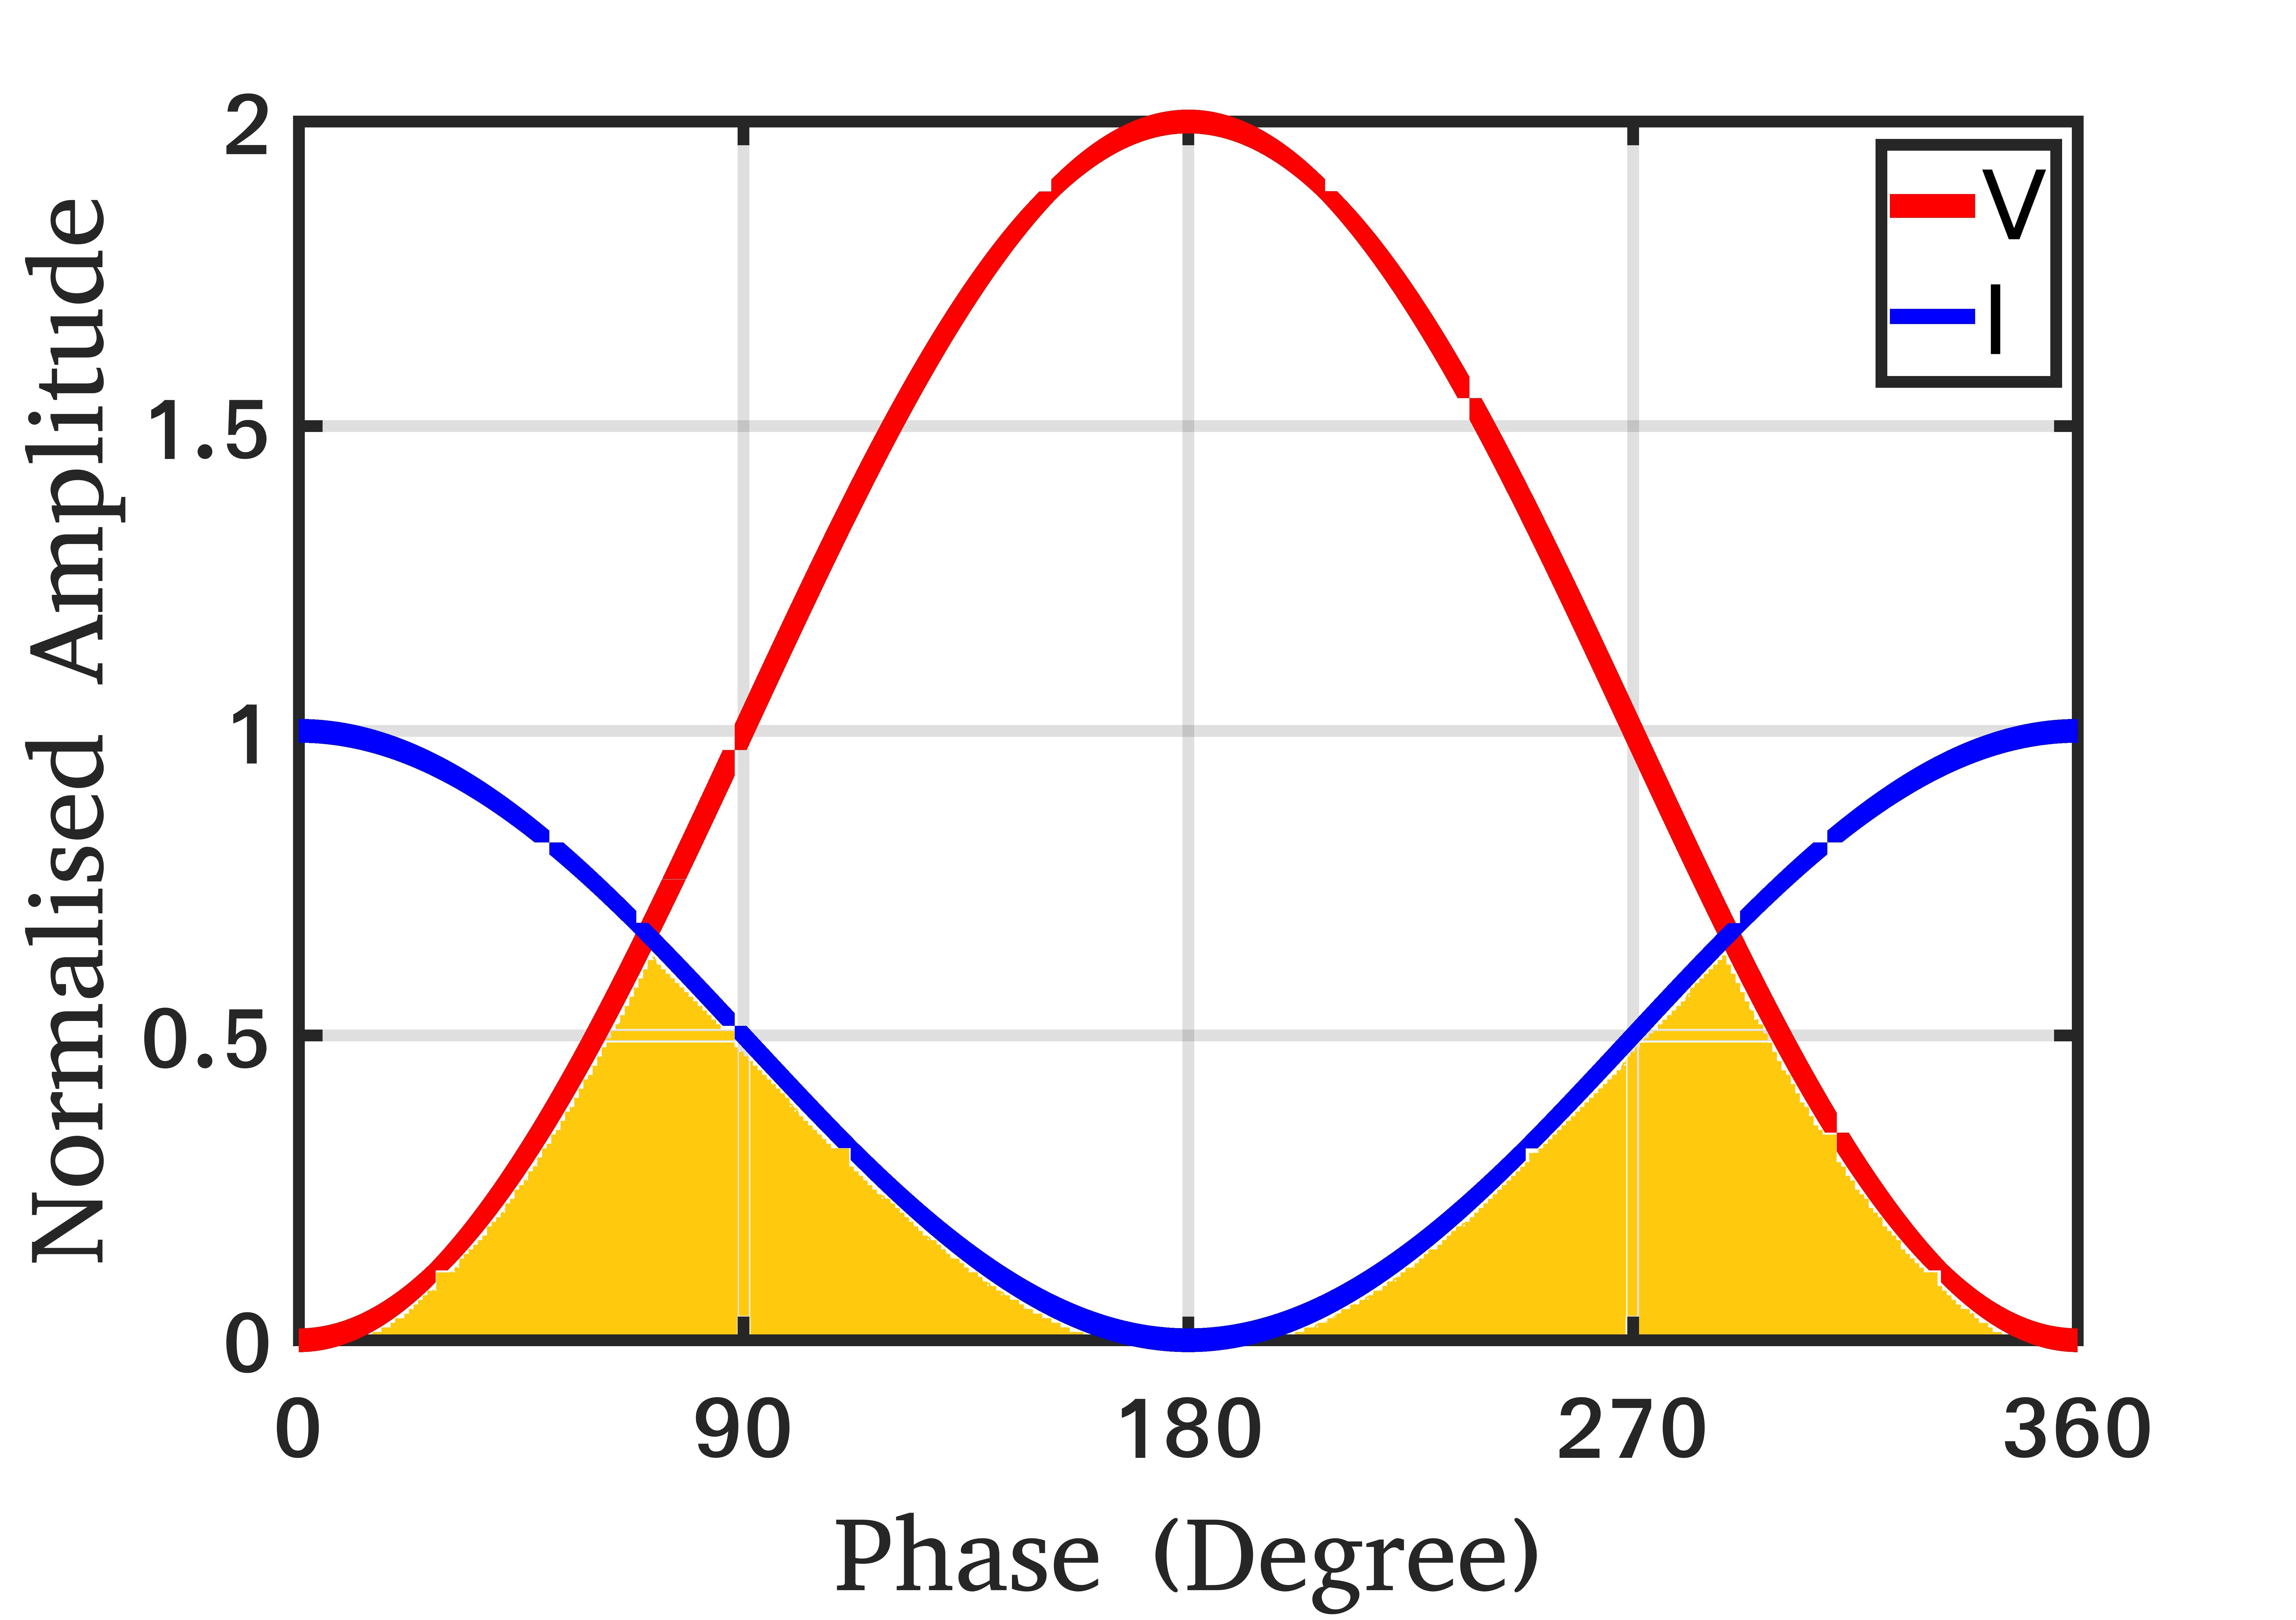
\includegraphics[width=0.9\textwidth]{Images/Intro/ClassA_shaded.jpg}
\caption{Class A}
\label{fig:CA_wave_VI}
\end{subfigure}
\begin{subfigure}{0.24\textwidth}
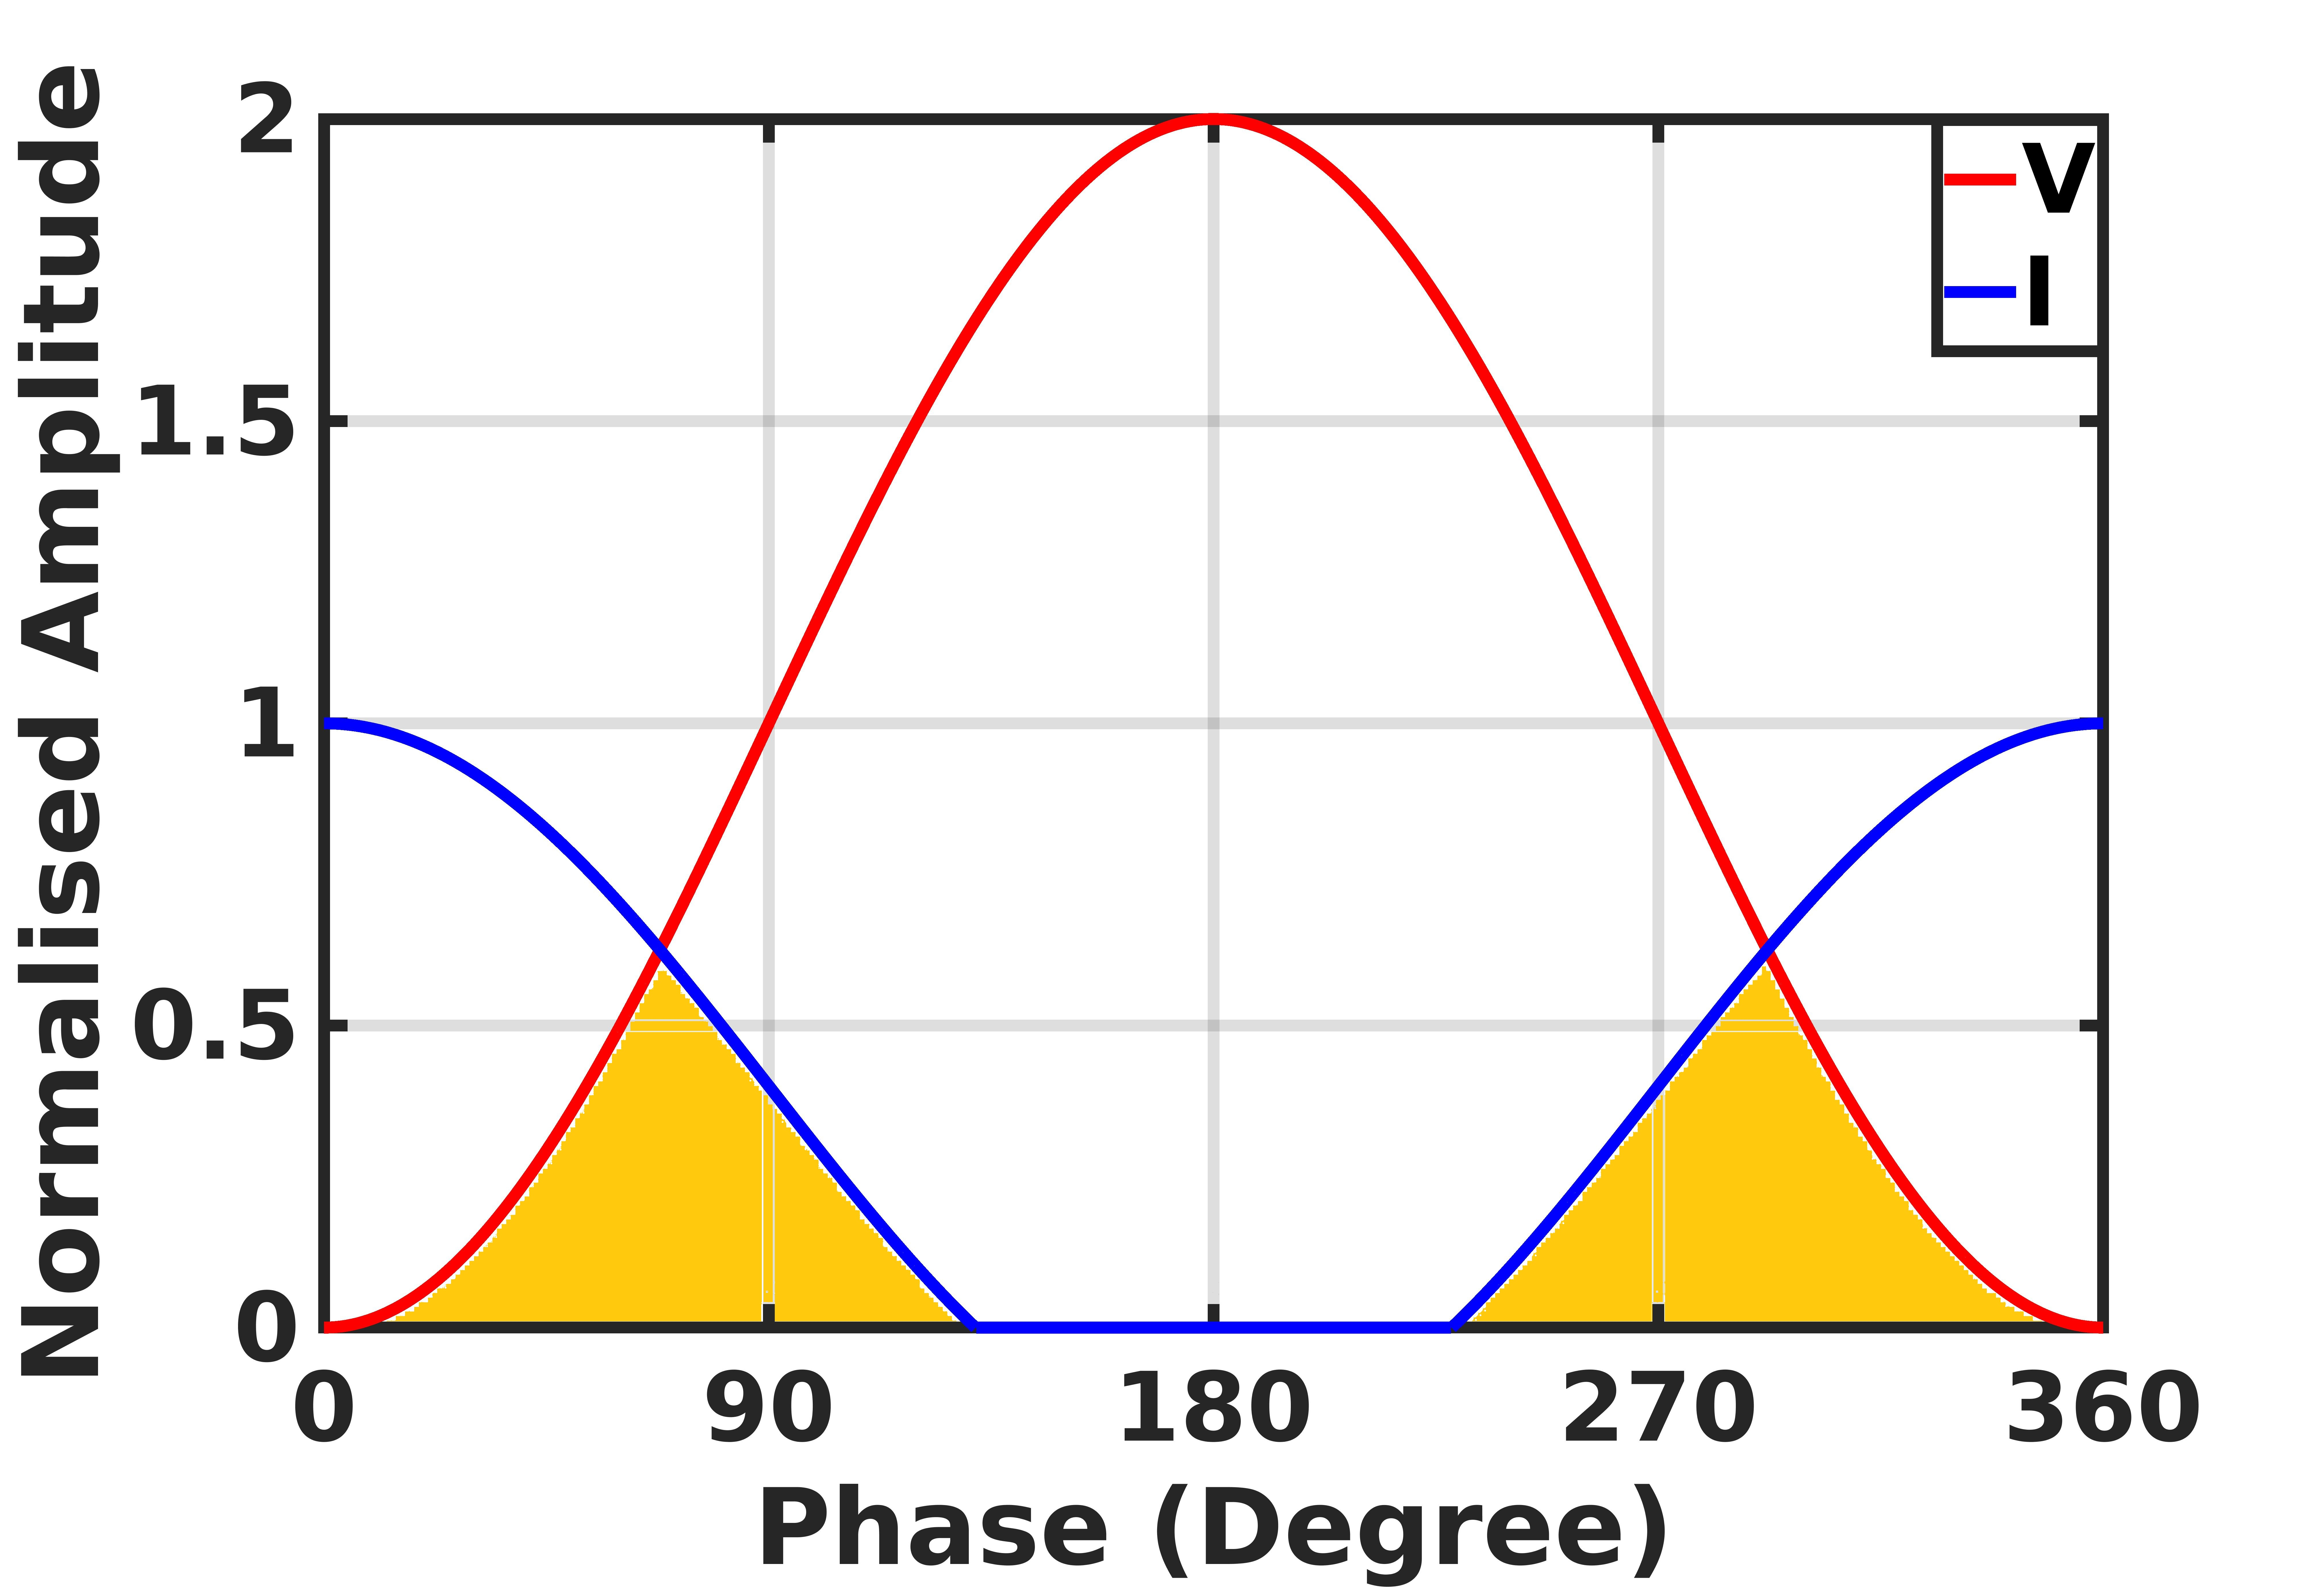
\includegraphics[width=0.9\textwidth]{Images/Intro/ClassB_shaded.jpg}
\caption{Class B}
\label{fig:CB_wave_VI}
\end{subfigure}
\begin{subfigure}{0.24\textwidth}
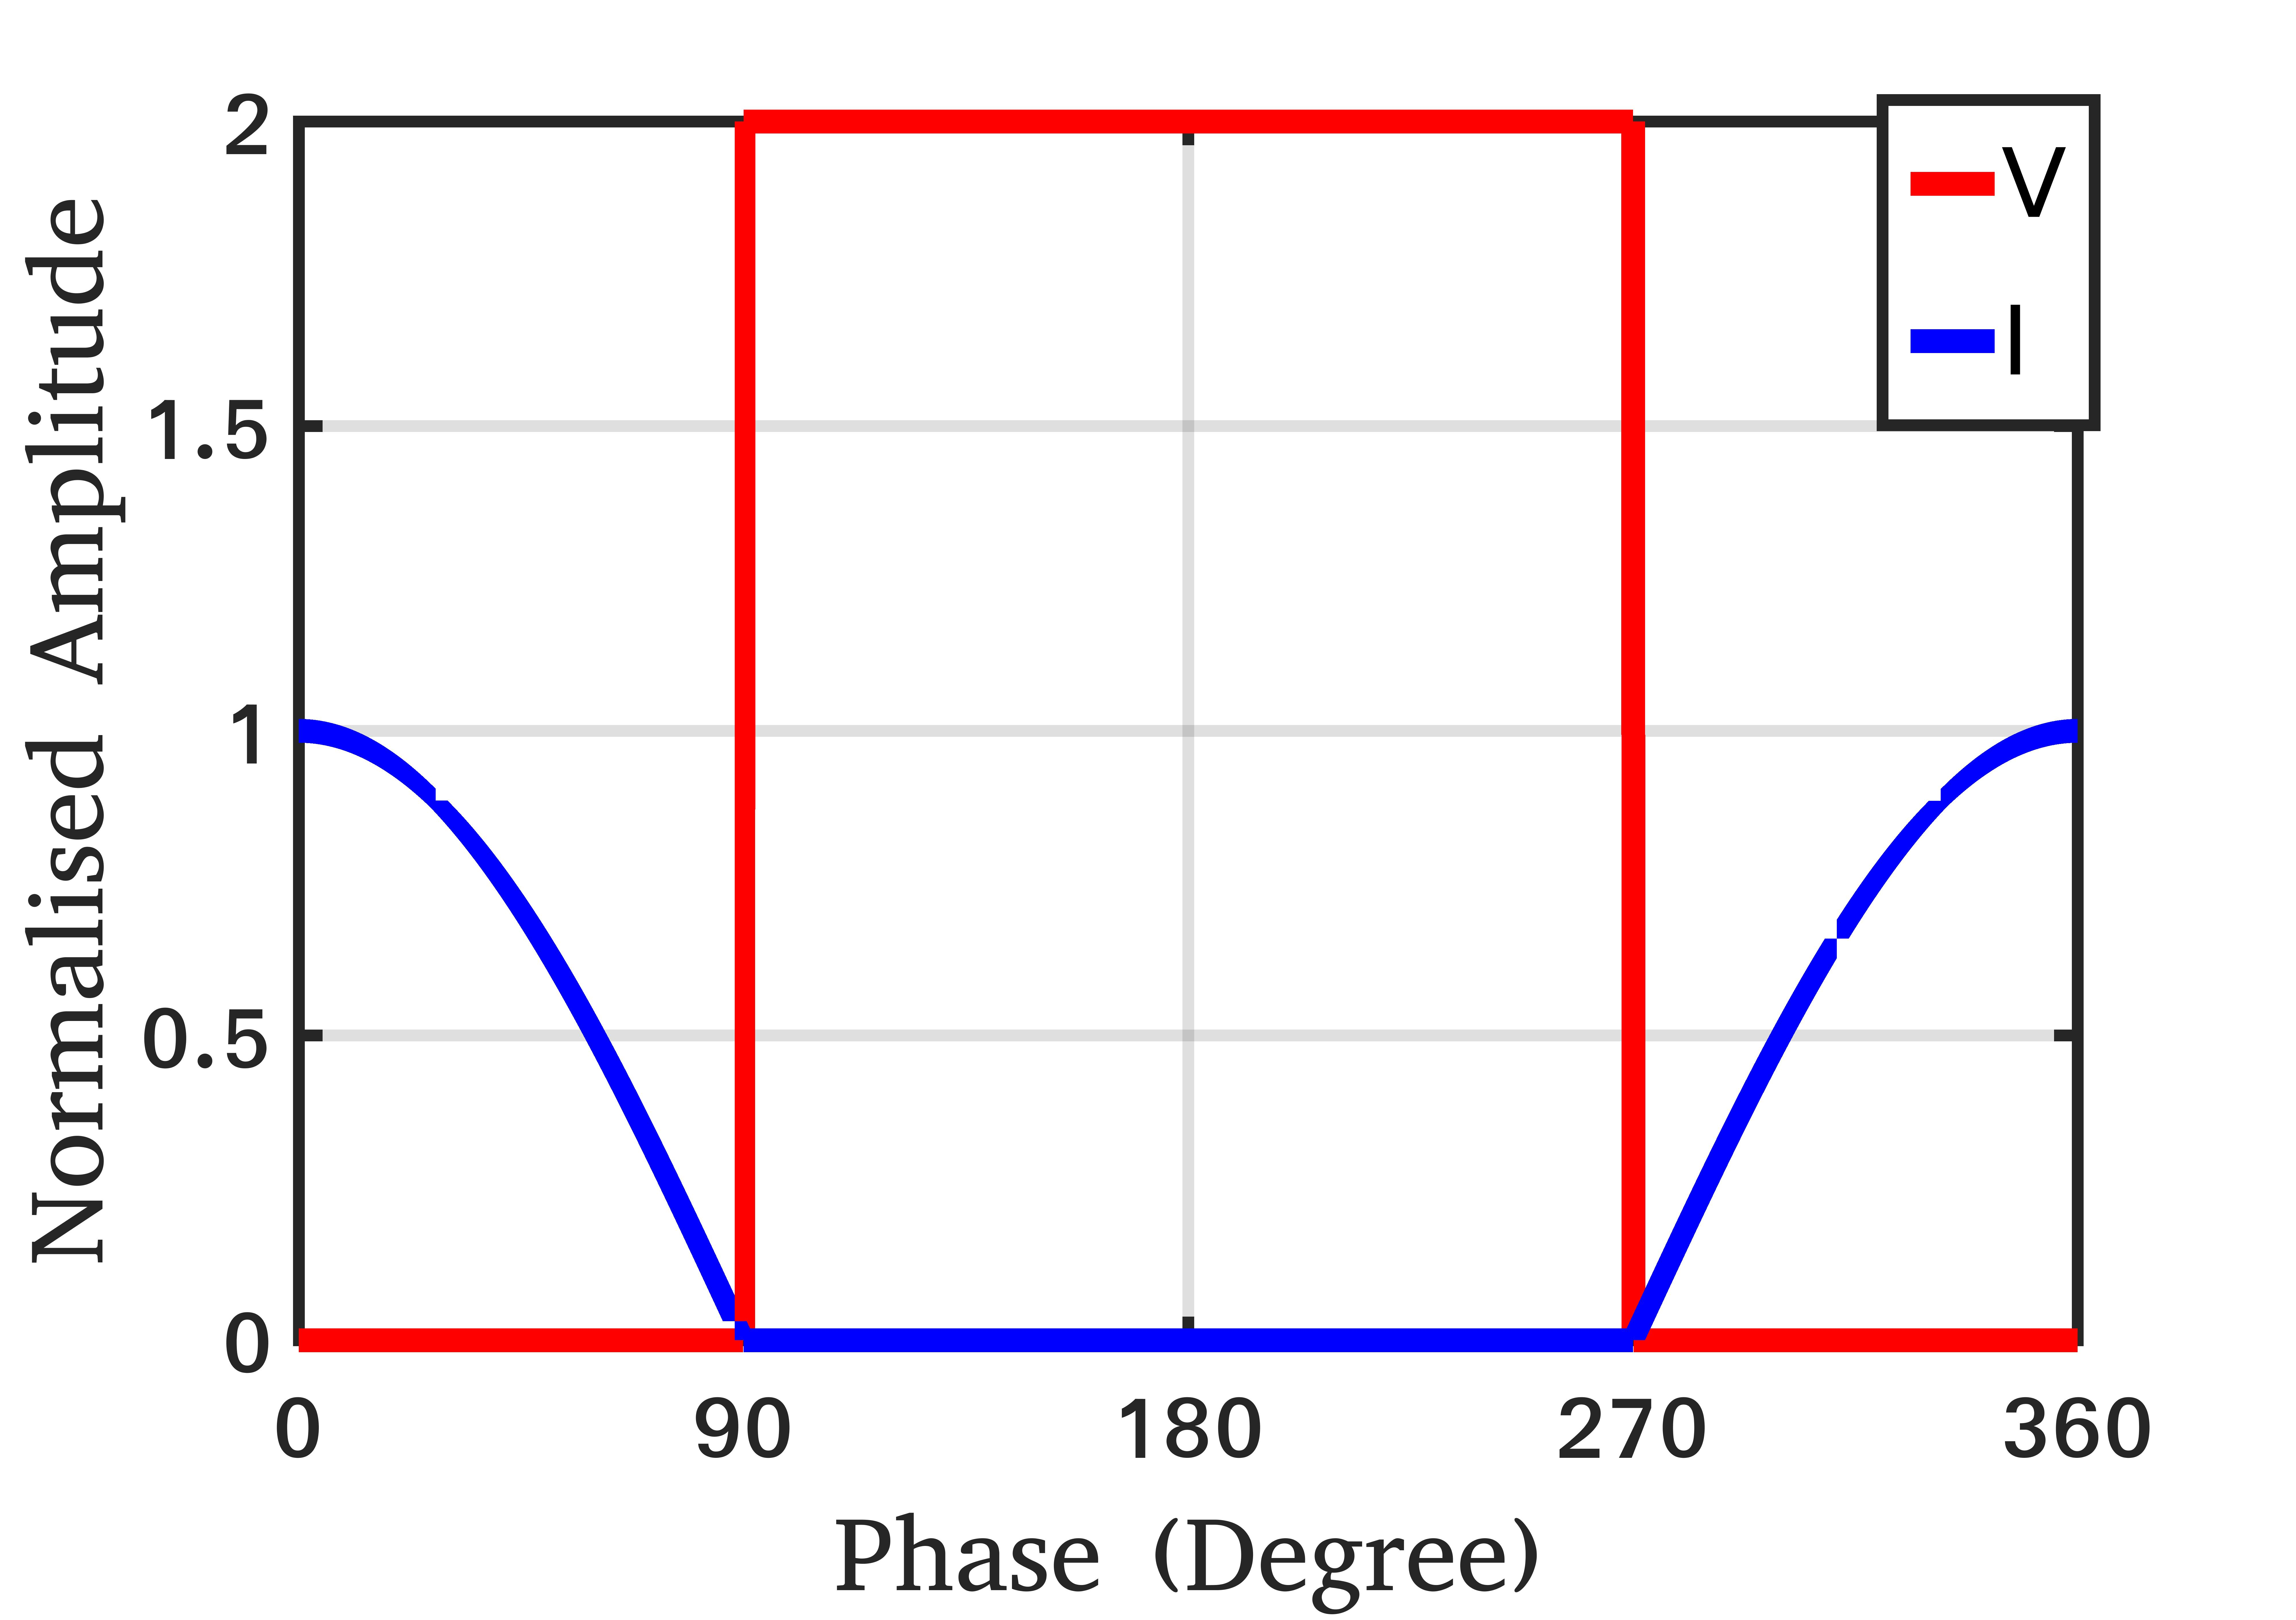
\includegraphics[width=0.9\textwidth]{Images/Intro/ClassF.jpg}
\caption{Ideal Class F}
\label{fig:ICF_wave_VI}
\end{subfigure}
\begin{subfigure}{0.24\textwidth}
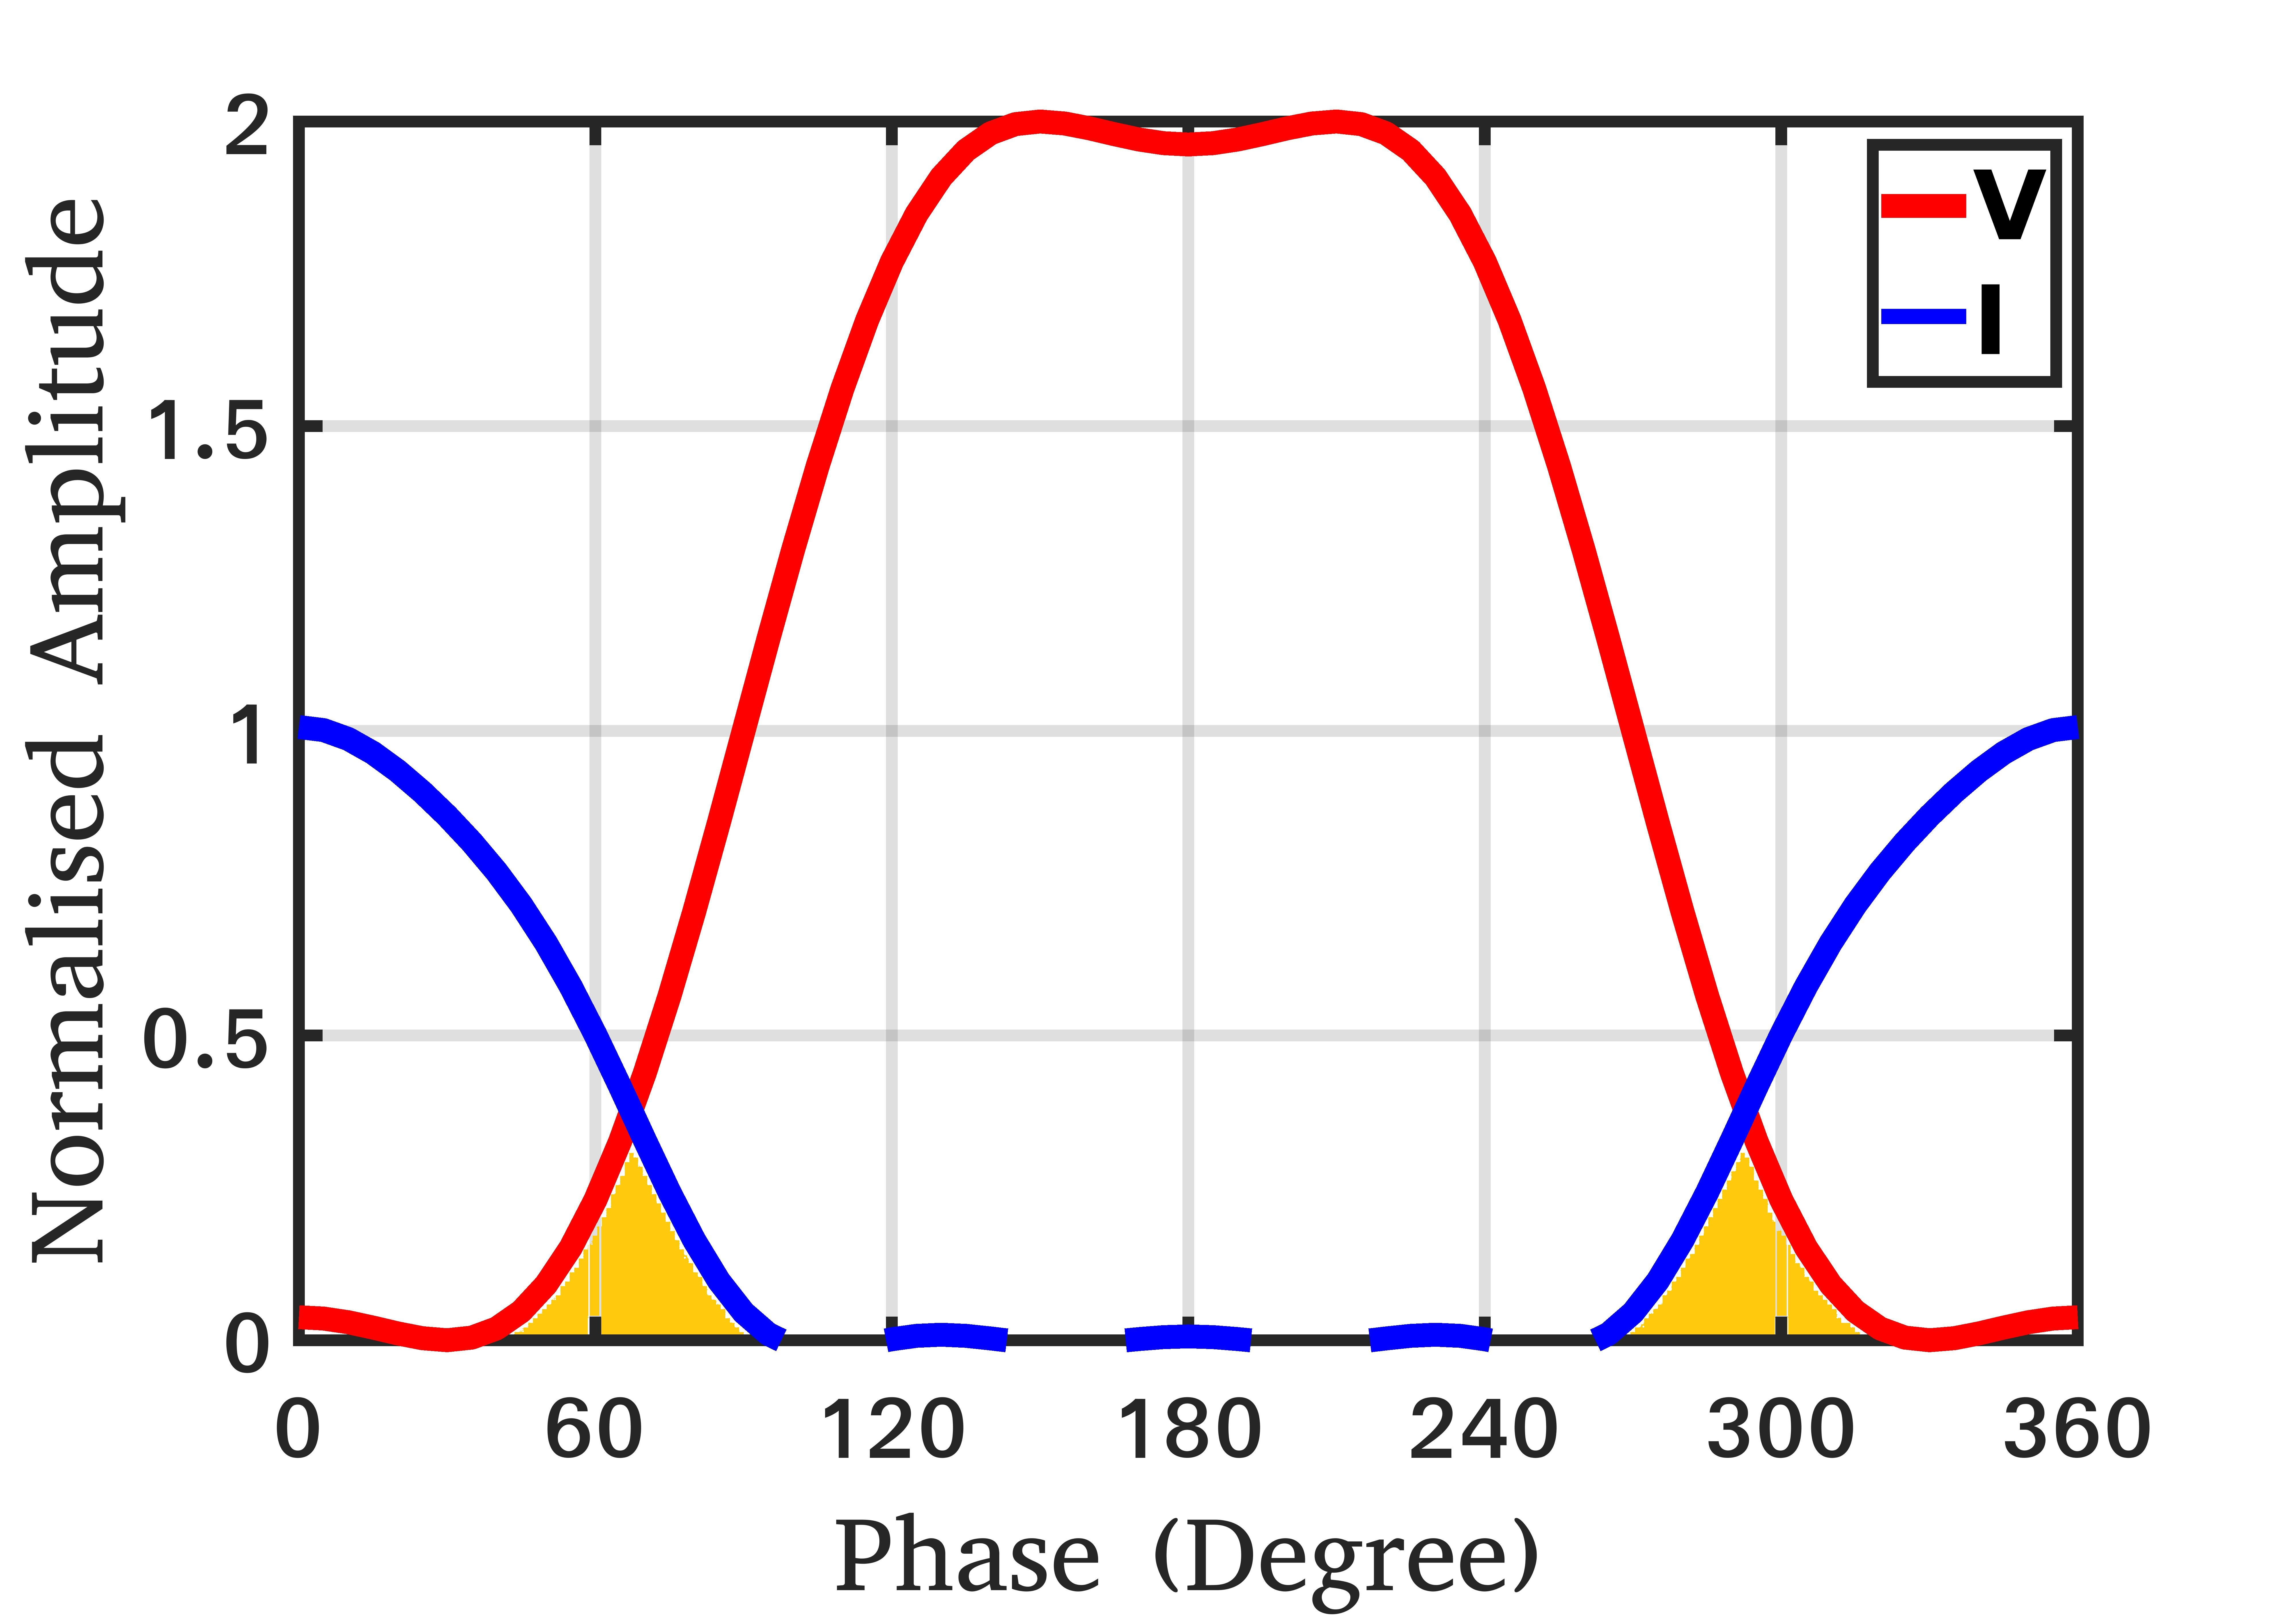
\includegraphics[width=0.9\textwidth]{Images/Intro/CF_wave_VI_shaded.jpg}
\caption{Practical Class F}
\label{fig:CF_wave_VI}
\end{subfigure}
\caption{The class A/B/F drain  voltage (V)/current (I) waveforms. \color{black}}
\label{fig:wave_VI}
\vspace{-0.25in}
\end{figure}
Generalized drain source\color{blue}-\color{black}voltage ($V_{DS}$) containing all frequencies up to $3^{rd}$ harmonic \cite{Gen_Vds_eqn} is given by:
\begin{equation}
V_{DS}=\underbrace{1}_{\text{DC}}-\underbrace{\frac{2}{\sqrt{3}} \cos \theta}_{\text{fundamental}}+\underbrace{\frac{1}{3 \sqrt{3}} \cos 3 \theta}_{\text{$3^{rd}$ harmonic}}
\label{eqn_CF_V}
\end{equation}
The drain current ($I_{D}$), which is a half-sine wave, is given by
\begin{equation}
I_{D}=\underbrace{\frac{1}{\pi}}_{\text{DC}}+\underbrace{\frac{1}{2} \cos \theta}_{\text{fundamental}}+\underbrace{\frac{2}{3 \pi} \cos 2 \theta}_{\text{$2^{nd}$ harmonic}}-\underbrace{\frac{2}{15 \pi} \cos 4 \theta}_{\text{$4^{th}$ harmonic}}
\label{eqn_CCF_I}
\end{equation}
The load impedance at the fundamental, $2^{nd}$ and $3^{rd}$ harmonic are represented by $Z_{1f}$, $Z_{2f}$, and $Z_{3f}$, respectively.
\begin{equation}
\begin{aligned}
Z_{1f}=\frac{4}{\sqrt{3}}, \hspace{3mm}
Z_{2f}=0, \hspace{3mm}
Z_{3f}=\infty
\end{aligned}
\label{eqn_CF}
\end{equation}
As depicted in Fig. \ref{fig:CF_wave_VI},  one of the advantages of class F PAs is that its normalized peak drain voltage is two. Nonetheless, they suffer from limited operational bandwidth (typically \textit{10\%}) owing to the need for short and open circuit harmonic terminations. Thus, to realize wider bandwidth, the continuous class F (CCF) PA has been proposed \cite{CCF_reason}.

In this paper, we propose an on-chip CCF output stage network. This paper is organized as follows. Section \ref{section:CCF} briefly explains the equations governing the operation of CCF. Section \ref{section:ON} discusses the design procedure of different CCF output networks. Section \ref{section:Results} compares the proposed four output stages, and Section \ref{section:Conclusion} concludes this paper.

\section{Continuous Class F}
\label{section:CCF}
\vspace{-0.05in}
Compared to class F, the CCF has an imaginary part added at the fundamental and $2^{nd}$ harmonic of the voltage waveform. Thus, the generalized $V_{DS}$ for CCF is given by \cite{ECCF_Carrubba}:
\begin{equation}
V_{DS}=\underbrace{1}_{\text{DC}}-\underbrace{\frac{2}{\sqrt{3}} \cos \theta-\gamma \sin \theta}_{\text{fundamental}}+\underbrace{\frac{7 \gamma}{6 \sqrt{3}} \sin 2 \theta}_{\text{$2^{nd}$ harmonic}}+\underbrace{\frac{1}{3 \sqrt{3}} \cos 3 \theta}_{\text{$3^{rd}$ harmonic}}
\label{eqn_CCF_V}
\end{equation}
As in class F, $I_{D}$ is a half sinusoid (given in (\ref{eqn_CCF_I})). These equations indicate that $V_{DS}$/$I_{D}$ are chosen in such a way that no power is dissipated at higher harmonics. Also, mathematically, the $\gamma$ in (\ref{eqn_CCF_V}) does not affect drain efficiency ($\eta_D$). But it affects the peak drain voltage, as depicted in Fig. \ref{fig:CCF_wave_VI}. In reality, however, $I_{D}$ depends on $V_{DS}$, degrading $\eta_D$ as $\gamma$ increases.

\begin{figure}[!t]
\centering
\captionsetup{font=footnotesize}
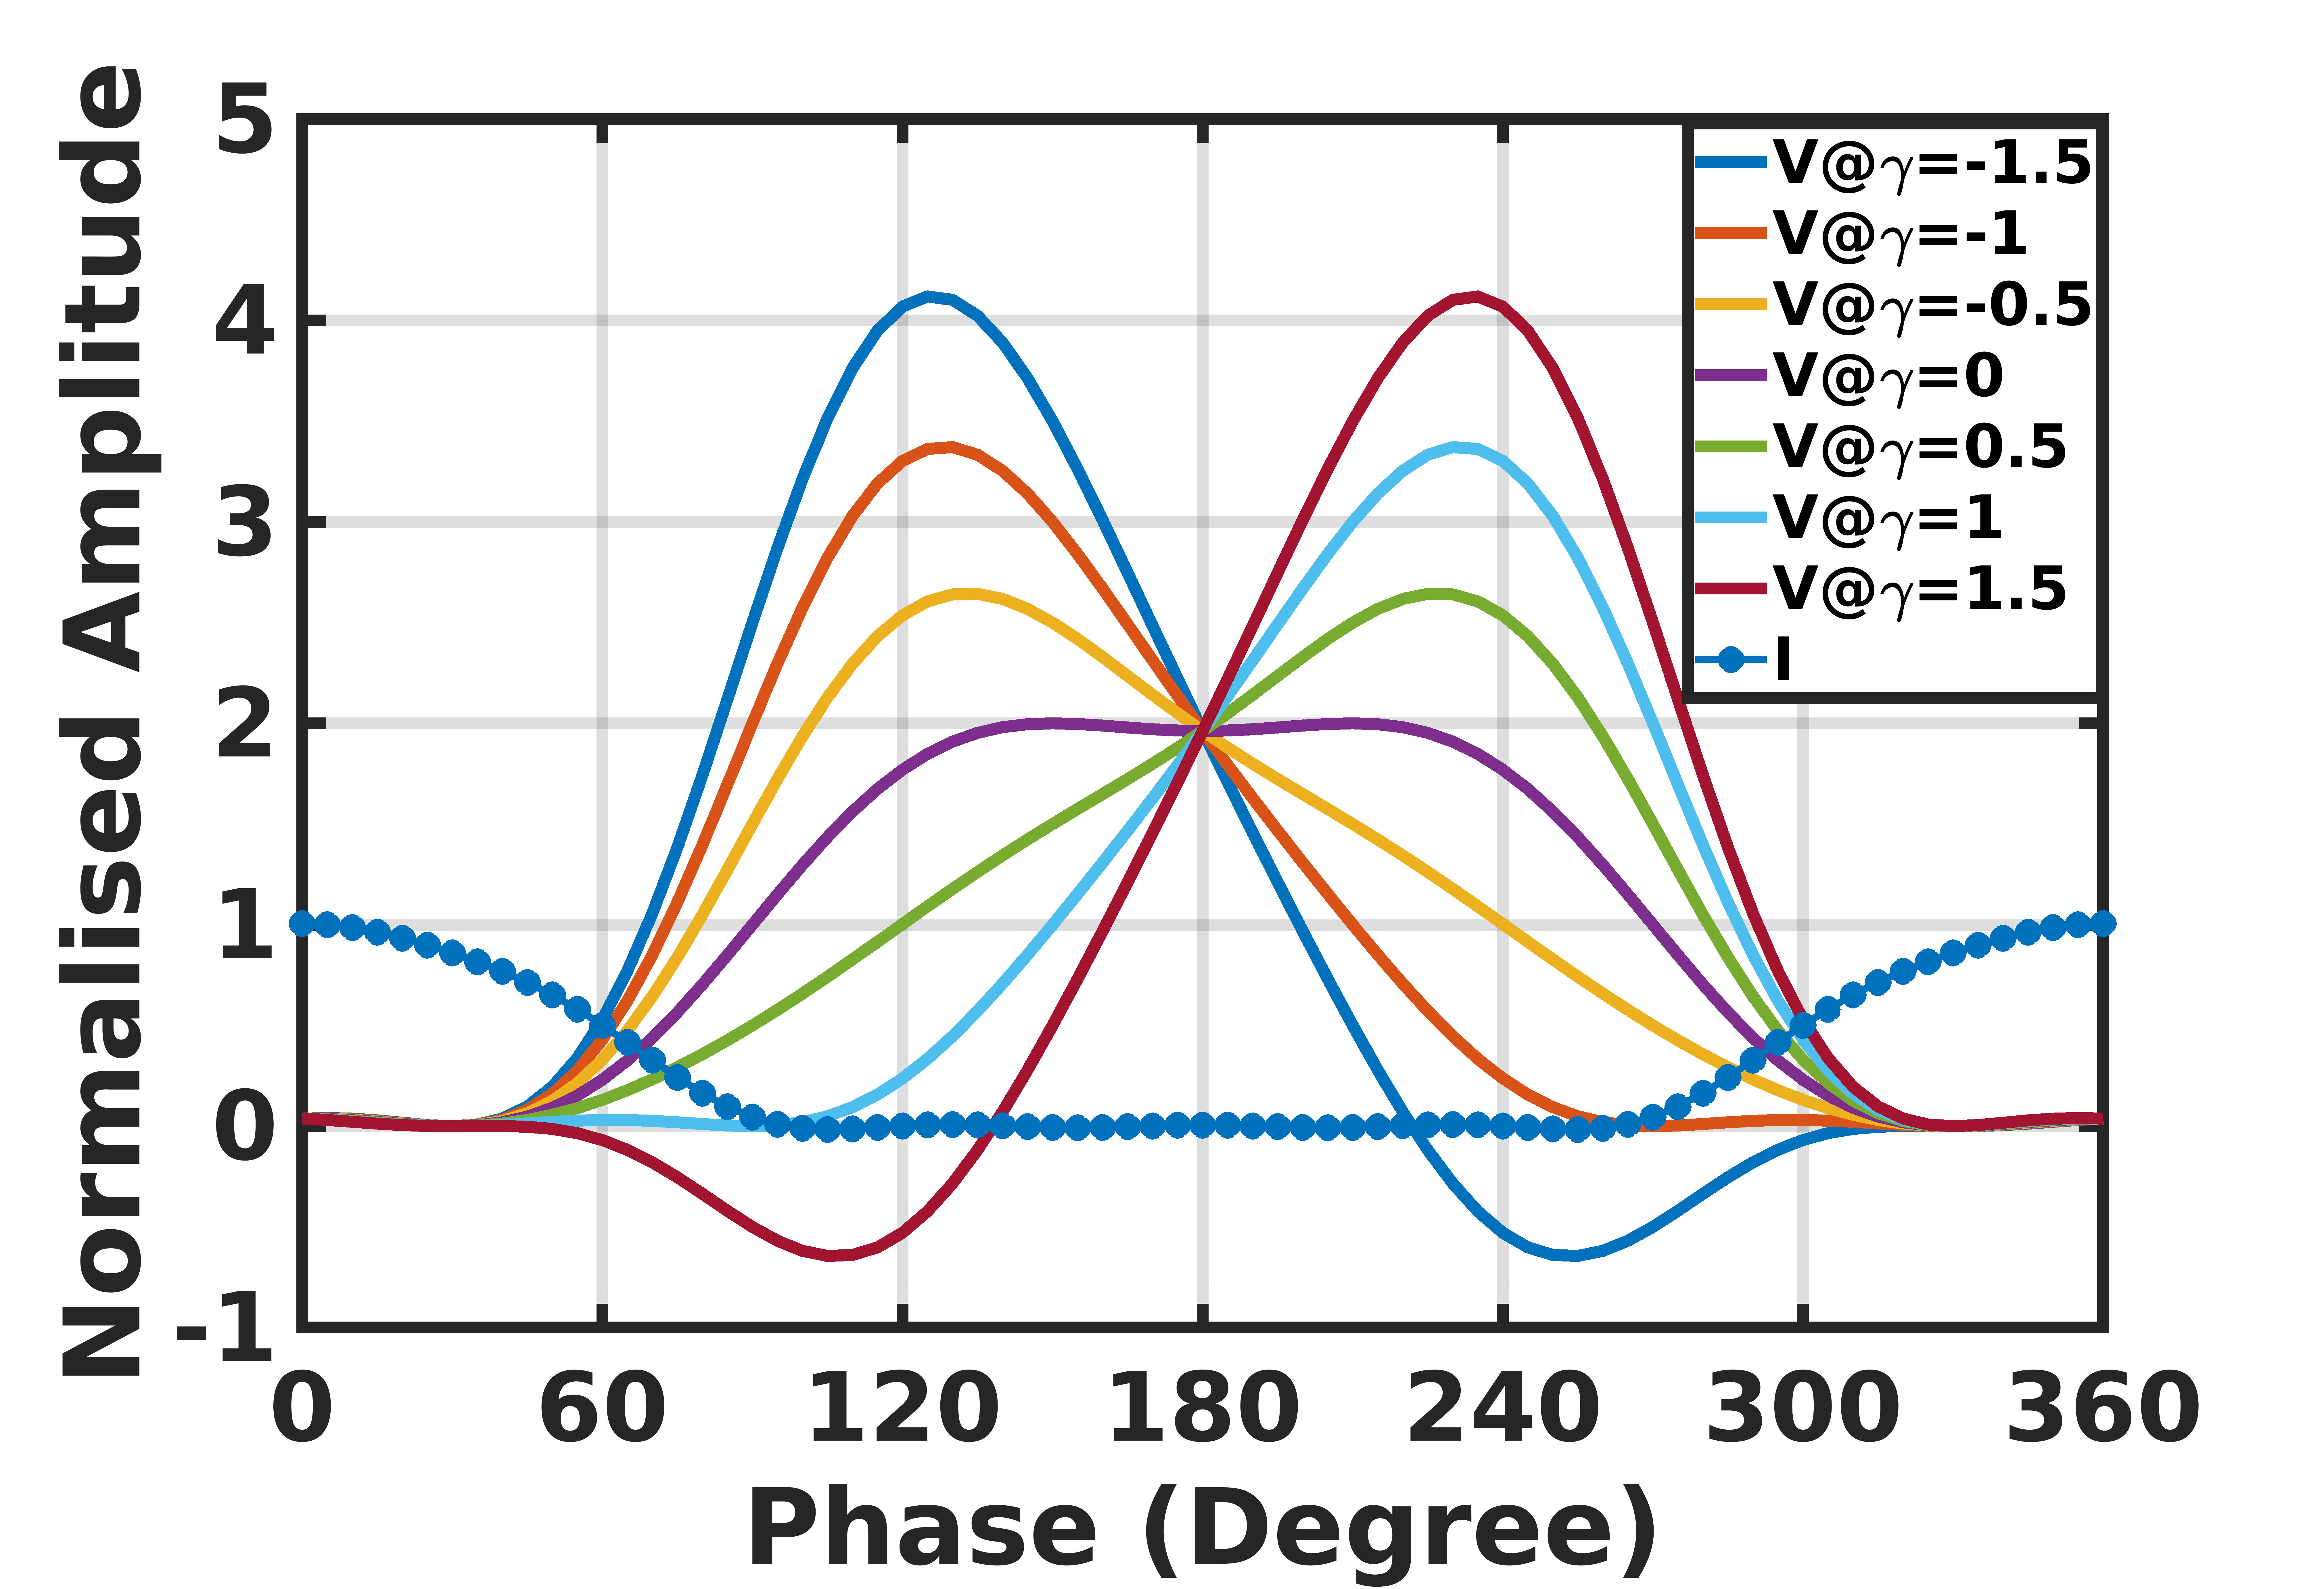
\includegraphics[width=3.4in, height=2in]{Images/CCF/CCF_wave_VI.jpg}
\caption{$V_{DS}$ and $I_D$ waveform for CCF with \textit{-1.5} $<$ $\gamma$ $<$ \textit{1.5}.}
\label{fig:CCF_wave_VI}
\vspace{-0.25in}
\end{figure}

Fig. \ref{fig:CCF_wave_VI} implies that at $\gamma$ = \textit{0}, waveform is like class F. For the $\gamma$ values between \textit{-1} and \textit{1}, $V_{DS}$ remains positive, enabling CCF PA to meet linearity requirements. However, CCF PAs suffer from large peak drain voltage which can be as high as \textit{3.12} times the supply ($V_{DD}$) when $\gamma$ = \textit{-1} or \textit{1}. Using (\ref{eqn_CCF_V}) and (\ref{eqn_CCF_I}), the load impedance of CCF  are calculated \cite{CCFDesign_ali}.
\begin{equation}
\begin{aligned}
Z_{1f}=\frac{4}{\sqrt{3}}+j 2 \gamma, \hspace{2mm}
Z_{2f}=0-j \frac{\pi}{2} \frac{7 \sqrt{3}}{6} \gamma,\hspace{2mm}
Z_{3f}=\infty
\label{eqn_CCF_imp}
\end{aligned}
\end{equation}

In CCF, $Z_{3f}$ remains open-circuited similar to class F. Meanwhile, $Z_{1f}$ and $Z_{2f}$ have a reactive part, unlike class F. From (\ref{eqn_CCF_imp}) and Fig. \ref{fig:CCF_SC}, it is observed that if the reactive part of $Z_{1f}$ changes from inductive to capacitive, then the reactive part of $Z_{2f}$  needs to change from capacitive to inductive or vice-versa across the bandwidth to achieve CCF operation. In the next section, the design procedure for the proposed four output networks is meticulously explained. 

\begin{figure}[!t]
\centering
\captionsetup{font=footnotesize}
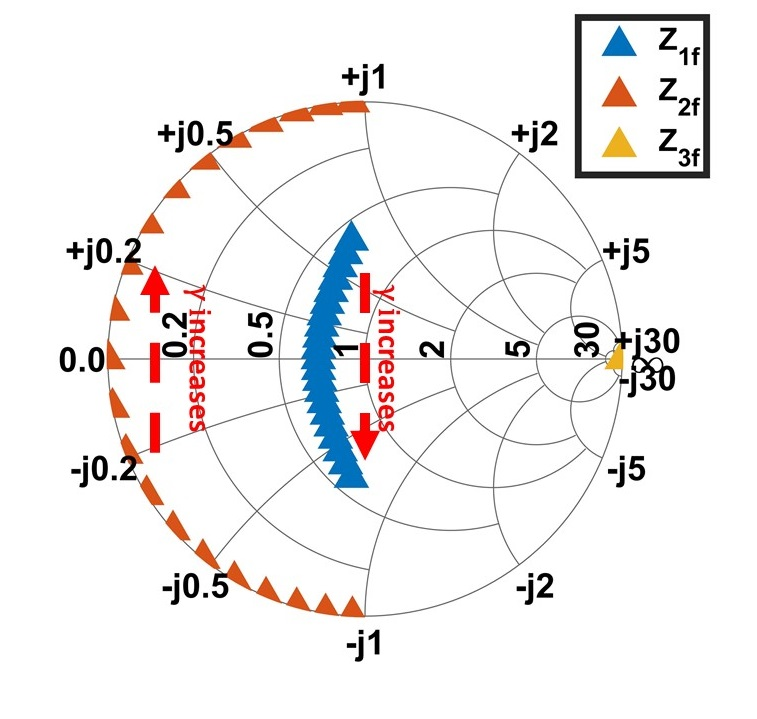
\includegraphics[width=0.63\linewidth]{Images/CCF/CCF_SC.jpg}
\caption{Variation of $Z_{1f}$, $Z_{2f}$, $Z_{3f}$ for \textit{-1} $<$ $\gamma$ $<$ \textit{1}.}
\label{fig:CCF_SC}
\vspace{-0.05in}
\end{figure}
 

\section{Design of Output Network for CCF}
\label{section:ON}
In this paper, the push-pull (differential) structure is chosen for the PA mainly because it decouples the odd harmonics ($1^{st}$/$3^{rd}$) from even harmonic ($2^{nd}$) impedance. Moreover, it suppresses supply/substrate noise and second-order nonlinearities as well as doubles the RF output power. 
In this work, the targeted peak RF power is \textit{27 dBm}  while its operational bandwidth is \textit{2.1 -- 2.7 GHz} with $V_{DD}$ = \textit{2.7 V}. To achieve this, a  fundamental differential impedance of \textit{38.7} $\Omega$ should be presented to the drains of the transistors across the \textit{2.1 -- 2.7 GHz} band, which is obtained as follows:
\vspace{-0.05in}
\begin{equation}
\begin{aligned}
&V_{FUND}(de)=2*V_{FUND}(se)=2*\frac{2}{\sqrt{3}} V_{DD}=6.24 \hspace{1mm}V\\
&R_{D}(de)=\frac{V_{FUND}(de)^{2}}{2*\text{Peak} \hspace{1mm} P_{OUT}}=38.7 \hspace{1mm} \Omega
\label{eqn_diff_imp}
\end{aligned}
\end{equation}
The requirements of the output network for CCF is exhibited in Tab. \ref{tab:Output_Network_Requirements}. The PA operates in class F mode at the center frequency $\omega_0$ (\textit{2.4 GHz}) with a short at $2\omega_0$ (\textit{4.8 GHz}) and an open at $3\omega_0$ (\textit{7.2 GHz}). But, for all other frequencies, the PA performs in the CCF mode. 

\setlength{\arrayrulewidth}{0.5mm}
\setlength{\tabcolsep}{2pt}
\renewcommand{\arraystretch}{1.5}
\begin{table}[!t]
\centering
\captionsetup{font=footnotesize}
\resizebox{\linewidth}{!}{%
\begin{tabular}{|c|c|c|c|}
\hline
\begin{tabular}[c]{@{}c@{}}\textbf{Class of} \\\textbf{Operation}\end{tabular} & \begin{tabular}[c]{@{}c@{}}\textbf{First Harmonic} \\($\omega$)\end{tabular} & \begin{tabular}[c]{@{}c@{}}\textbf{Second Harmonic} \\(2$\omega$)\end{tabular} & \begin{tabular}[c]{@{}c@{}}\textbf{Third Harmonic} \\(3$\omega$)\end{tabular} \\ \hline
\multirow{2}{*}{\textbf{\begin{tabular}[c]{@{}c@{}}Class F \\ (2.4 GHz)\end{tabular}}} & $\Re(Z_D)$ = 38.7 $\Omega$ & $\Re(Z_D)$= 0 $\Omega$ & \multirow{2}{*}{\begin{tabular}[c]{@{}c@{}}$|Z_D|\approx$ 1000 $\Omega$\end{tabular}} \\ \cline{2-3}
 & $\Im(Z_D)$ = 0 $\Omega$ & $\Im(Z_D)$ = 0 $\Omega$ &  \\ \hline
\multirow{2}{*}{\textbf{\begin{tabular}[c]{@{}c@{}}\\CCF \\ (2.1 - 2.7 GHz)\end{tabular}}} & $\Re(Z_D)$ = 38.7 $\Omega$ & $\Re(Z_D)$ = 0 $\Omega$ & \multirow{2}{*}{\begin{tabular}[c]{@{}c@{}}\\$|Z_D|\approx$ 1000 $\Omega$ \end{tabular}} \\ \cline{2-3}
 & \begin{tabular}[c]{@{}c@{}}$\Im(Z_D)$ $\rightarrow$ + to -\\ OR\\ $\Im(Z_D)$ $\rightarrow$ - to +\end{tabular} & \begin{tabular}[c]{@{}c@{}} $\Im(Z_D)$ $\rightarrow$ - to +\\ OR\\ $\Im(Z_D)$ $\rightarrow$ + to -\end{tabular} &  \\ \hline
\end{tabular}%
 }
\caption{Output network specifications.}
\label{tab:Output_Network_Requirements}
\vspace{-0.25in}
\end{table}

The proposed four different  output networks, which are designed using lossless lumped components, are illustrated in Fig. \ref{fig:Design_A_FC} and \ref{fig:Design_B_C_D}a/b/c. 
All the designs consist of a balun and a load capacitance ($C_L$). The balun converts the balanced (differential) signal to its single-ended companion, whereas $C_L$ adjusts $3^{rd}$ harmonic impedance. The power transistor's drain-source capacitance (assume $C_{DS}=1.87\hspace{1mm}pF$) is absorbed into the output network to reduce its impact on the PA performance. The balun is modeled using an ideal transformer, comprising of magnetizing inductance ($L_m$), leakage inductance ($L_k$), primary inductance ($L_P$), and coupling coefficient ($km$) \cite{Transformer_model}. 

\subsection{Design A (no RF choke \& with $L_2C_2$)}
Design A consists of a second harmonic trap ($L_2C_2$), which provides short at $2\omega_0$. The $V_{DD}$ is  supplied through the balun's center tap and $L_{BND}$ is used to model bond-wire inductance ($\approx$ \textit{1 nH}).
Analysis of the schematics is performed in differential-/common-mode scenarios by utilizing the equivalent circuits depicted in Fig. \ref{fig:Design_A}b/c, respectively to calculate the unknown parameters: transformer's coupling factor ($km$) and turn ratio ($N$) along with  $L_P$, $C_2$, $L_2$, and $C_L$.

\begin{figure}[!t]
\captionsetup{font=footnotesize}
\centering
\begin{subfigure}{0.5\textwidth}
\centering
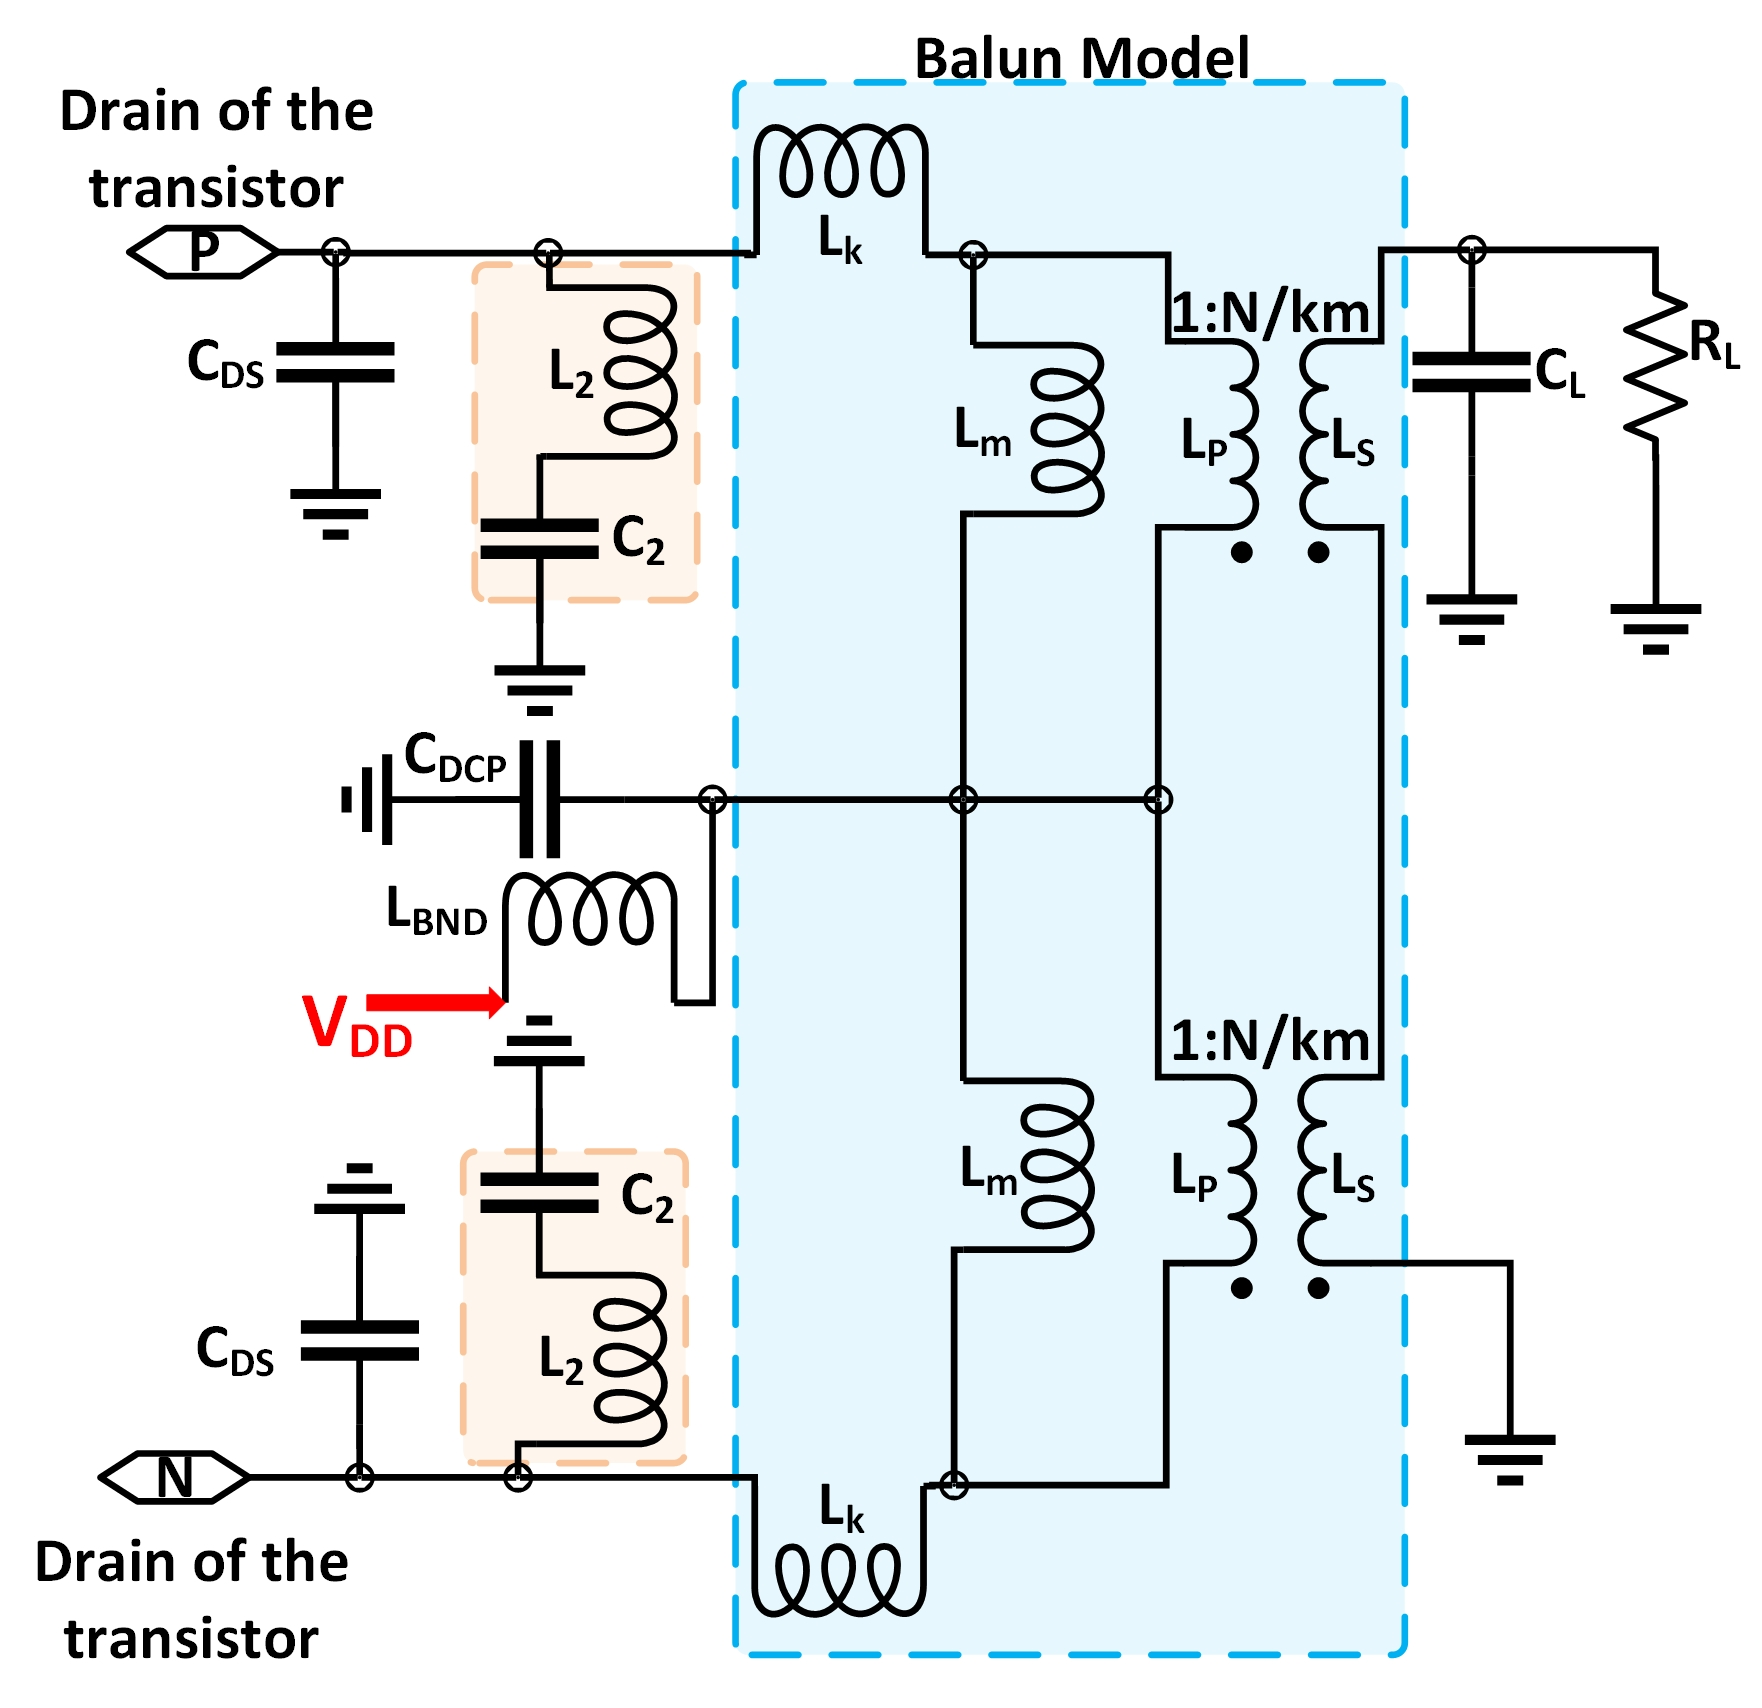
\includegraphics[width=0.4\textwidth]{Images/Design/Design_A_FC.jpg}
\caption{}
\label{fig:Design_A_FC}
\end{subfigure}
\begin{subfigure}[b]{0.24\textwidth}
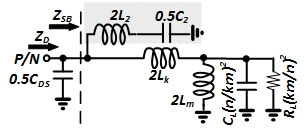
\includegraphics[width=1\textwidth]{Images/Design/Design_A_Diff.jpg}
\caption{}
\label{fig:Design_A_Diff}
\end{subfigure}
\begin{subfigure}[b]{0.24\textwidth}
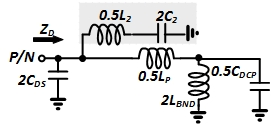
\includegraphics[width=0.9\textwidth]{Images/Design/Design_A_Com.jpg}
\caption{}
\label{fig:Design_A_Com}
\end{subfigure}
\caption{(a) Design A (Balun, $L_2C_2$ and $C_L$), (b) differential-mode, and (c) common-mode equivalent circuit }
\label{fig:Design_A}
\vspace{-0.2in}
\end{figure}

Fig. \ref{fig:Design_A_Diff} shows that the drain impedance ($Z_D$) is given by
\vspace{-0.05in}
\begin{equation}
    Z_D=(\frac{1}{\frac{j\omega C_{DS}}{2}}+\frac{1}{Z_{SB}})^{-1}=38.7 \hspace{1mm} \Omega
    \label{eqn:ZD}
\end{equation}
The value of $Z_{SB}$ (impedance of $L_2C_2$ and balun given by (\ref{eqn:Design_A_ZSB})) that will provide $Z_D$ of \textit{38.7} $\Omega$ can be calculated from (\ref{eqn:ZD}) and the value is $\Re(Z_{SB})(\omega_0) =  29.8\hspace{1mm} \Omega$ and $\Im(Z_{SB})(\omega_0) = 16.6\hspace{1mm}\Omega$.
\vspace{-0.05in}
\begin{equation}
\begin{aligned}
    &Z_{SB}=(\frac{1}{Z_B}+\frac{1}{Z_S})^{-1}
    \hspace{1mm}\text{where}, Z_S=2j\omega  L_2+\frac{1}{\frac{j \omega C_2}{2}}, \\
    &Z_B=(\frac{1}{R_P}+\frac{1}{2j \omega  L_m}+j \omega C_P)^{-1}+2j \omega  L_k,\\ &R_P=R_L(\frac{km}{n})^2,C_P=C_L(\frac{n}{km})^2
\label{eqn:Design_A_ZSB}
\end{aligned}
\end{equation}

It is evident from (7) that $C_{DS}$ should resonate with $\Im(Z_{SB})$ to attain high drain impedance at $3\omega_0$. This implies $\Im(Z_{SB})(3\omega_0) = 24.96\hspace{1mm}\Omega$. Ideally, $\Re(Z_{SB})(3\omega_0)$ should be \textit{0} to achieve high $3^{rd}$ harmonic impedance. However, Fig. \ref{fig:Design_A_Rn_var_1H} depicts that having a larger $\Re(Z_{SB)}(3\omega_0)$ contributes to a constant $P_{OUT}$ across the operational bandwidth by flattering the real part at the fundamental. Another benefit is that it has a  more linear reactive part at the fundamental, which is essential in CCF operation.
However, this leads to a lower $3^{rd}$ harmonic impedance, as showcased in Fig. \ref{fig:Design_A_Zn_3H}. This also emphasizes  the significance of $C_L$. Thus, to achieve \textit{1000} $\Omega$ at $3^{rd}$ harmonic,  $\Re(Z_{SB})(3\omega_0) = 0.5\hspace{1mm}\Omega$, which is obtained from Fig. \ref{fig:Design_A_Zn_3H}. Fig. \ref{fig:Design_A_Com} proves that $L_2$ should have a series resonance with $C_2$ to get short at 2$\omega_0$.

\vspace{-0.05in}
\begin{equation}
    L_2=\frac{1}{4*\omega_0^2*C_2}%=0.73 \hspace{1mm} nH
    \label{eqn:Design_A_2H}
\end{equation}

\begin{figure}[!t]
\captionsetup{font=footnotesize}
\centering
\begin{subfigure}{0.24\textwidth}
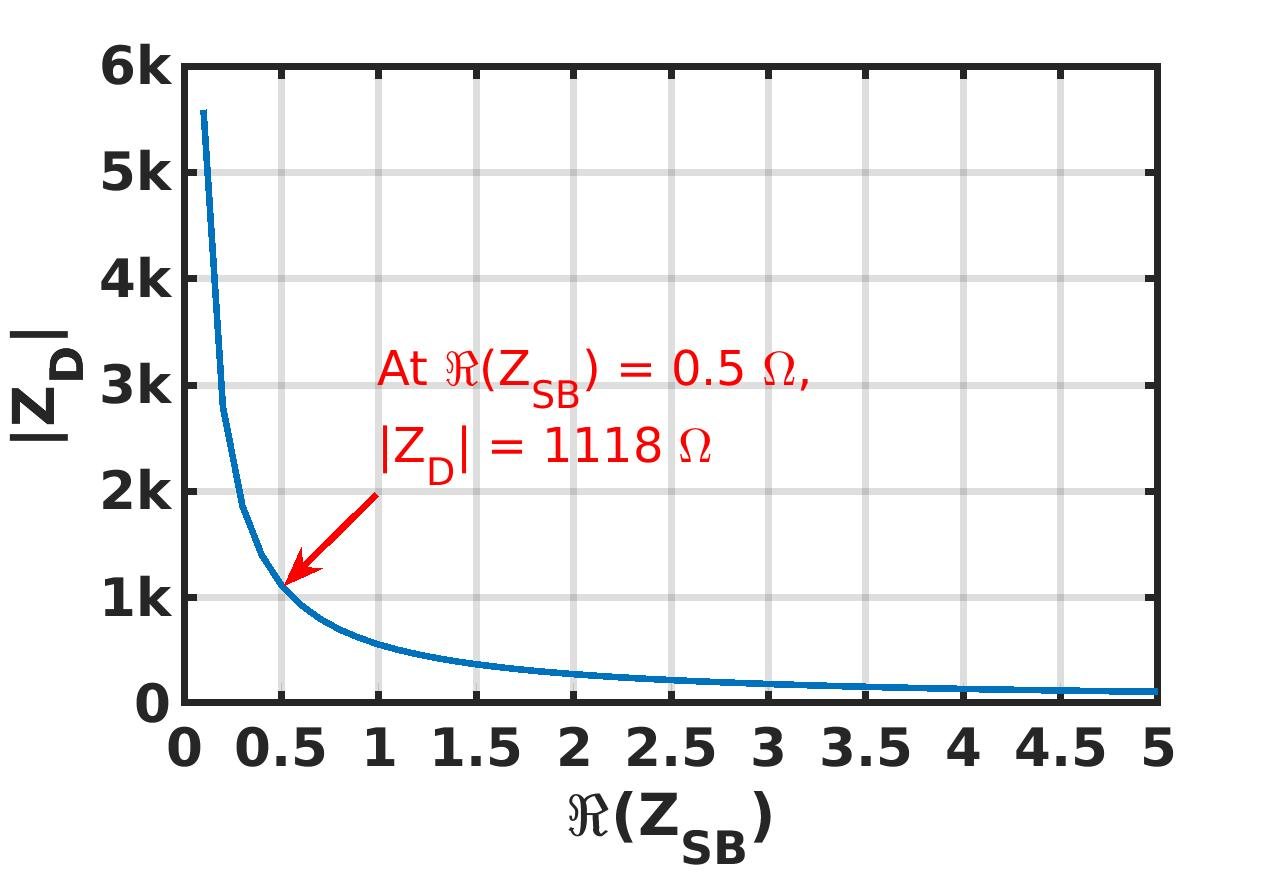
\includegraphics[width=1\textwidth]{Images/Design/Design_A_Zn_3H.jpg}
\caption{}
\label{fig:Design_A_Zn_3H}
\end{subfigure}
\begin{subfigure}{0.24\textwidth}
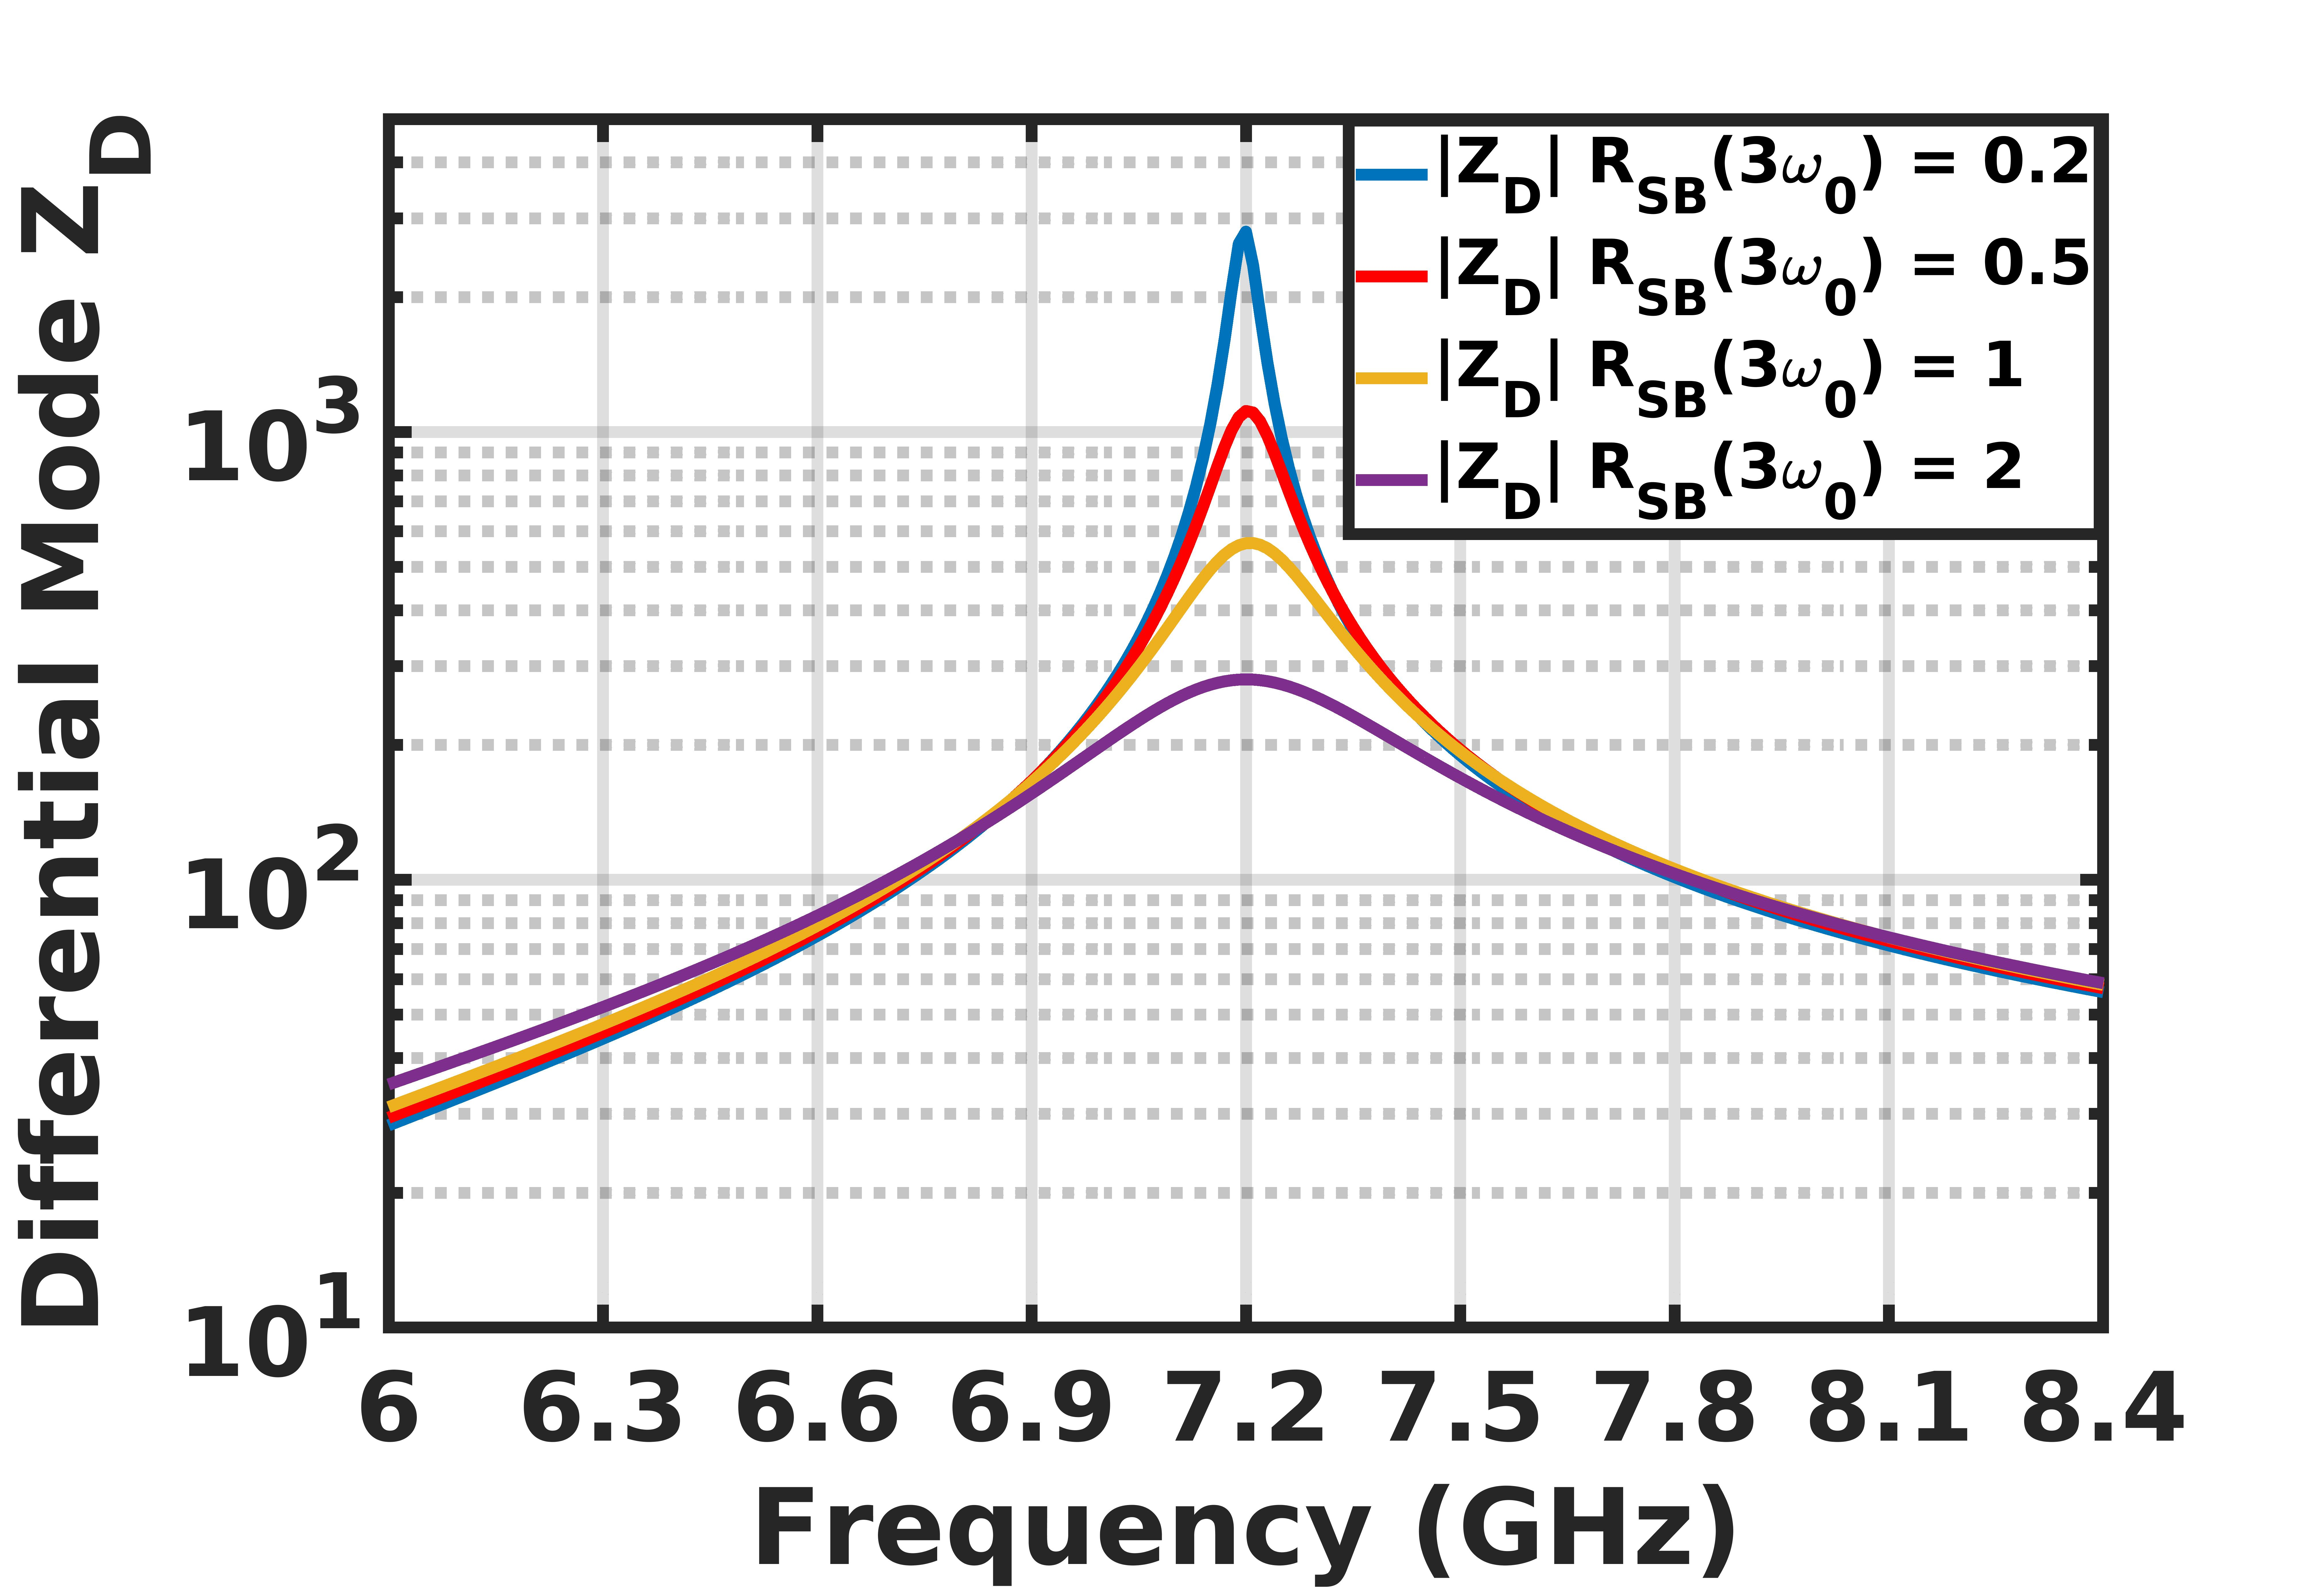
\includegraphics[width=1\textwidth]{Images/Design/Design_A_Rn_var_3H.jpg}
\caption{}
\label{fig:Design_A_Rn_var_3H}
\end{subfigure}
\begin{subfigure}{0.4\textwidth}
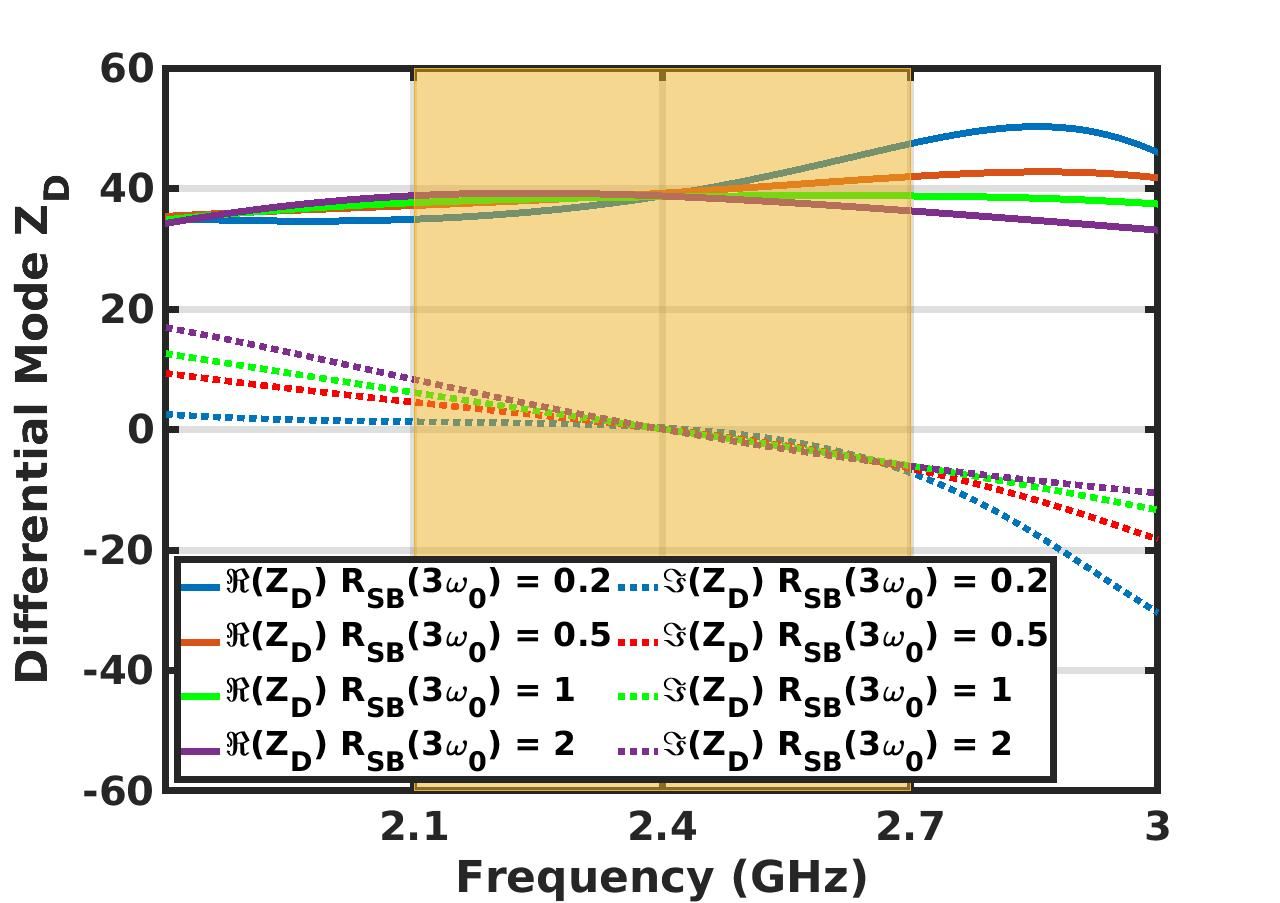
\includegraphics[width=1\textwidth]{Images/Design/Design_A_Rn_var_1H.jpg}
\caption{}
\label{fig:Design_A_Rn_var_1H}
\end{subfigure}
\caption{(a) Magnitude of $Z_{D}$ vs $\Re(Z_{SB})$ at $3\omega_0$, (b) Magnitude of $Z_D$ at $3^{rd}$ harmonic for various $R_{SB}(3\omega_0)$, and (c) $Z_D$ at fundamental for various $R_{SB}(3\omega_0)$.}
\label{fig:Design_A_Rn_var}
\vspace{-0.2in}
\end{figure}

The five unknowns in the circuit: $km$, $N$, $L_P$, $C_2$, and $C_L$ can be calculated by assuming one of them and using four equations ($\Re(Z_{SB})(\omega_0) =  29.8\hspace{1mm} \Omega$, $\Im(Z_{SB})(\omega_0) = 16.6\hspace{1mm}\Omega$, $\Re(Z_{SB})(3\omega_0) = 0.5\hspace{1mm}\Omega$ and  $\Im(Z_{SB})(3\omega_0) = 24.96\hspace{1mm}\Omega$). In this paper, $km =$ \textit{0.8} is assumed and the remaining unknowns ($N =$ \textit{1.34}, $L_P =$ \textit{2.2 nH}, $C_L =$ \textit{0.9 pF}, $C_2 =$ \textit{1.5 pF}, $L_2 =$ \textit{0.73 nH}) are calculated. The $km$ can be varied to get different sets of results in which $L_P$ is minimal and thereby making it layout friendly.


\subsection{Design B (no RF choke \& no $L_2C_2$)}

\begin{figure}[!t]
\captionsetup{font=footnotesize}
\centering
\begin{subfigure}{0.5\textwidth}
\centering
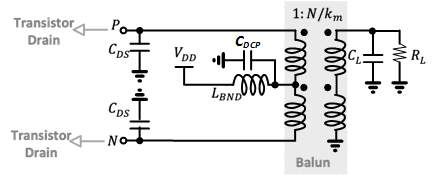
\includegraphics[width=0.4\textwidth]{Images/Design/Design_B_FC.jpg}
\caption{}
\label{fig:Design_B_FC}
\end{subfigure}
\begin{subfigure}{0.24\textwidth}
\centering
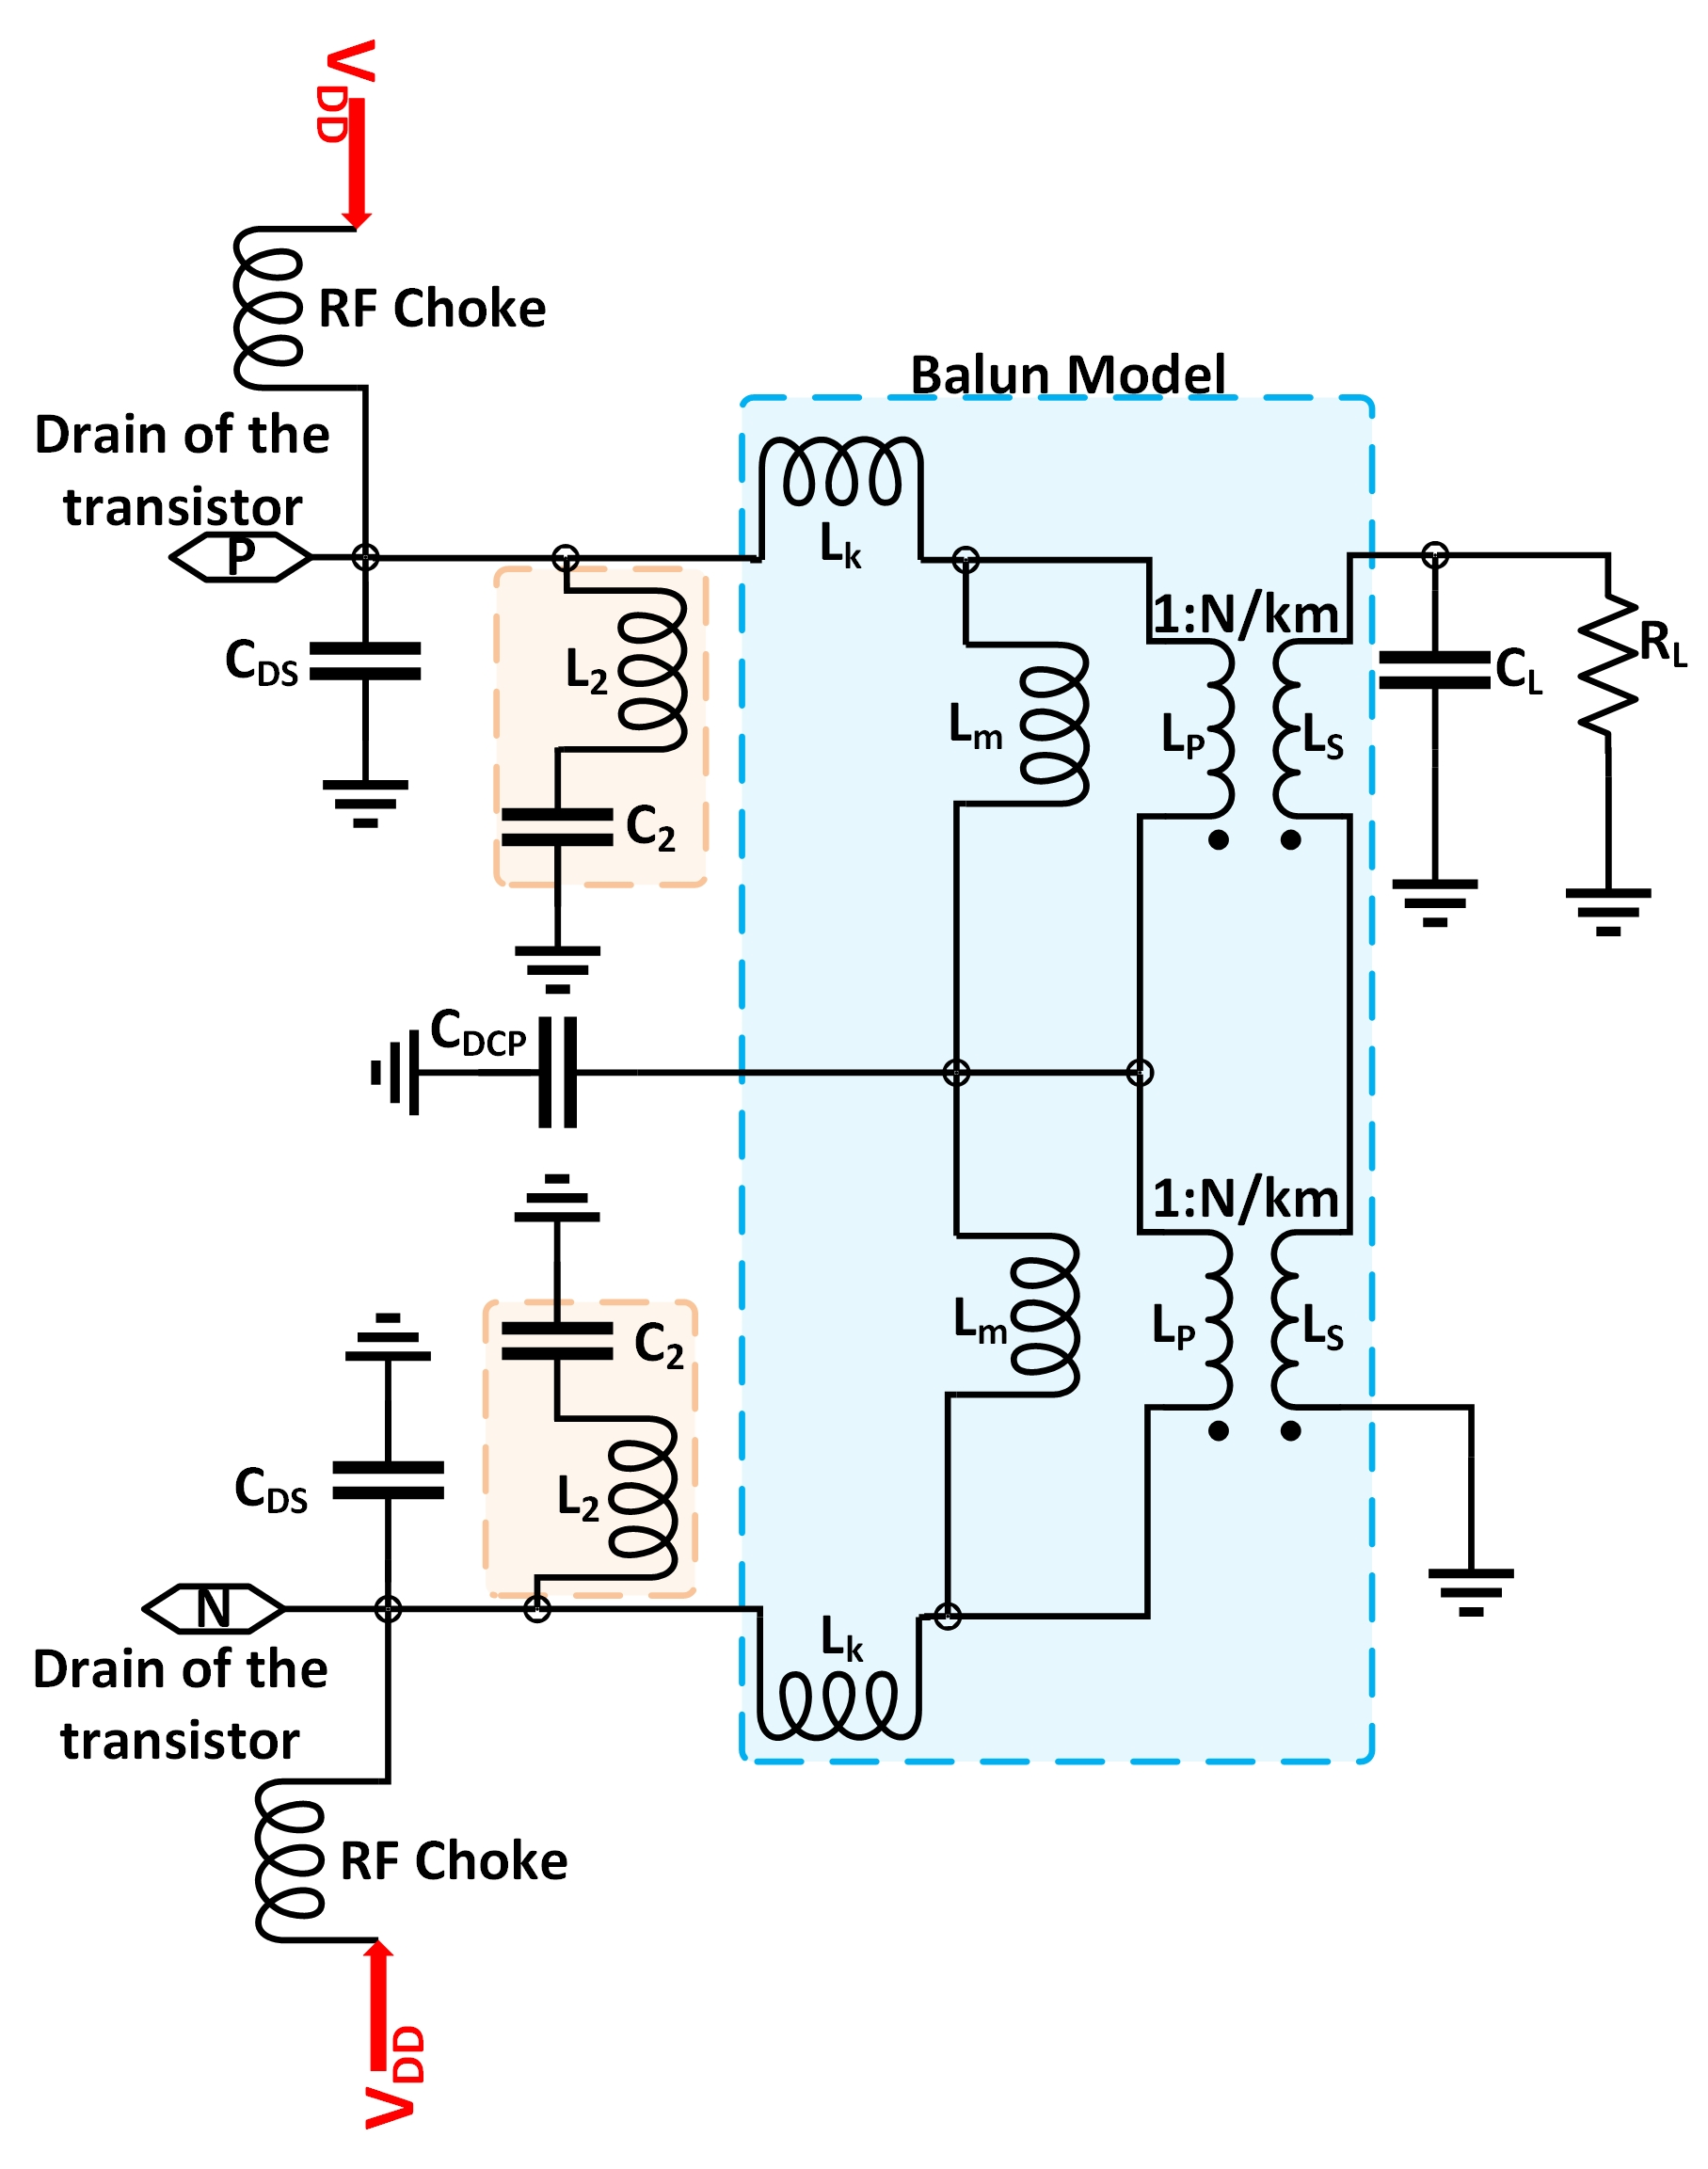
\includegraphics[width=0.8\textwidth]{Images/Design/Design_C_FC.jpg}
\caption{}
\label{fig:Design_C_FC}
\end{subfigure}
\centering
\begin{subfigure}{0.24\textwidth}
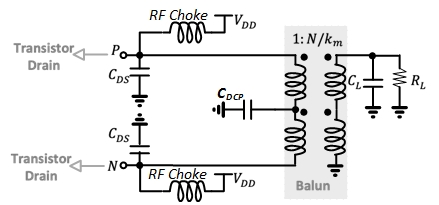
\includegraphics[width=0.8\textwidth]{Images/Design/Design_D_FC.jpg}
\caption{}
\label{fig:Design_D_FC}
\end{subfigure}
\caption{(a) Design B (Balun and $C_L$), (b) Design C (Balun, RF Choke, $L_2C_2$ \& $C_L$), and (c) Design D (Balun, RF Choke \& $C_L$).}
\label{fig:Design_B_C_D}
\vspace{-0.25in}
\end{figure}

In this design (Fig. \ref{fig:Design_B_FC}), $L_2C_2$ is removed, reducing the number of unknowns. Like the previous case, differential mode analysis yields four equations and there are four unknowns, thus leading to a single set of values for $km =$ \textit{0.72}, $N =$ \textit{0.9}, $L_P =$ \textit{0.63 nH}, $C_L =$ \textit{3.96 pF}, unlike design A. $C_{DCP}$ is tuned to provide a short at $2\omega_0$ such that $C_{DCP}$ resonates with $L_P$, $L_{BND}$, and $C_{DS}$, which is obtained from the common-mode analysis. Moreover, $C_{DCP}$ provides RF ground and blocks DC.

\subsection{Design C (with RF choke \& with $L_2C_2$)}
In this design (Fig. \ref{fig:Design_C_FC}), $V_{DD}$ is supplied through RF choke, unlike the previous designs. RF chokes are assumed to have a fixed value of \textit{5 nH}. The differential mode analysis yields four equations similar to design A. Assuming $km =$ \textit{0.8}, the other unknowns are calculated as $N =$ \textit{1.14}, $L_P =$ \textit{2.23 nH}, $C_L =$ \textit{1.10 pF}, $C_2 =$ \textit{1.37 pF}.
Like design A, $C_2$ should resonate out with $L_2$ to get short at $2\omega_0$. Thus, $L_2 =$ \textit{0.8 nH}. 

\subsection{Design D (with RF choke \& no $L_2C_2$)}
 Unlike design C, $L_2C_2$ is removed in this design (Fig. \ref{fig:Design_D_FC}). Also, RF choke should be calculated, assuming $C_{DS}$ resonates with it at $\omega_0$ (RF Choke = \textit{2.35 nH}).
The differential mode analysis yields four equations and the four unknowns ($N =$ \textit{0.84}, $L_P =$ \textit{0.86 nH}, $C_L =$ \textit{3.95 pF}, $km =$ \textit{0.77}) can be calculated.
$C_{DCP}$ can be tuned to provide a short at $2\omega_0$.

\section{Results}
\label{section:Results}

Fig. \ref{fig:Comp_1H_2H_3H}a/b show that all the four designs satisfying the main CCF requirements that are decreasing trend of the reactive part at the fundamental and increasing trend of the reactive part at $2^{nd}$ harmonic.
From Fig. \ref{fig:Comp_1H}, it is seen that the real part at the fundamental is flatter in the bandwidth \textit{2.1 -- 2.7 GHz} for design A and C, which, in turn, leads to constant $P_{OUT}$ in the specified bandwidth unlike design B and D. The $L_2C_2$, which acts as a varying capacitor at fundamental holds the reason for this. The designs B and D have a higher reactive part at the fundamental as compared to other designs, which in turn, leads to larger $\gamma$ value (refer (\ref{eqn_CCF_imp})) and thus, higher peak drain voltage (Fig. \ref{fig:CCF_wave_VI}). Fig. \ref{fig:Comp_1H_2H_3H}b/c show that all the four designs have similar response at $2^{nd}$ and $3^{rd}$ harmonic. 
%The impedance at \textit{2.1 GHz} and \textit{2.7 GHz} is less than \textit{200} $\Omega$ for all the \textit{4} designs.
So from the simulation, it is seen that design A outperforms other designs since it has the least number of components and more constant $P_{\text{OUT}}$ in the specified bandwidth.

\begin{figure}[!t]
\captionsetup{font=footnotesize}
\centering
\begin{subfigure}{0.5\textwidth}
\centering
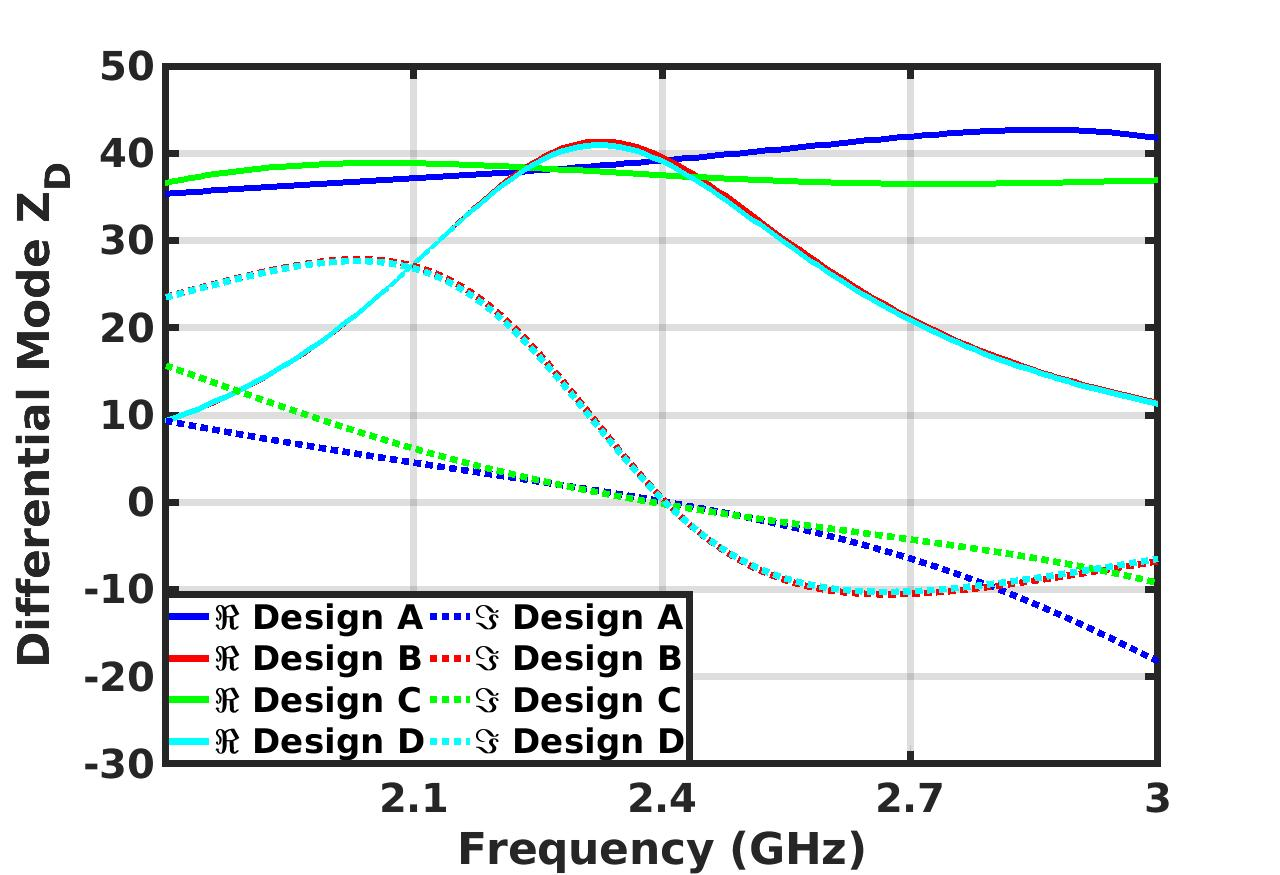
\includegraphics[width=0.65\textwidth]{Images/Output_Network_Comp/Comp_1H.jpg}
\caption{}
\label{fig:Comp_1H}
\end{subfigure}
\begin{subfigure}{0.24\textwidth}
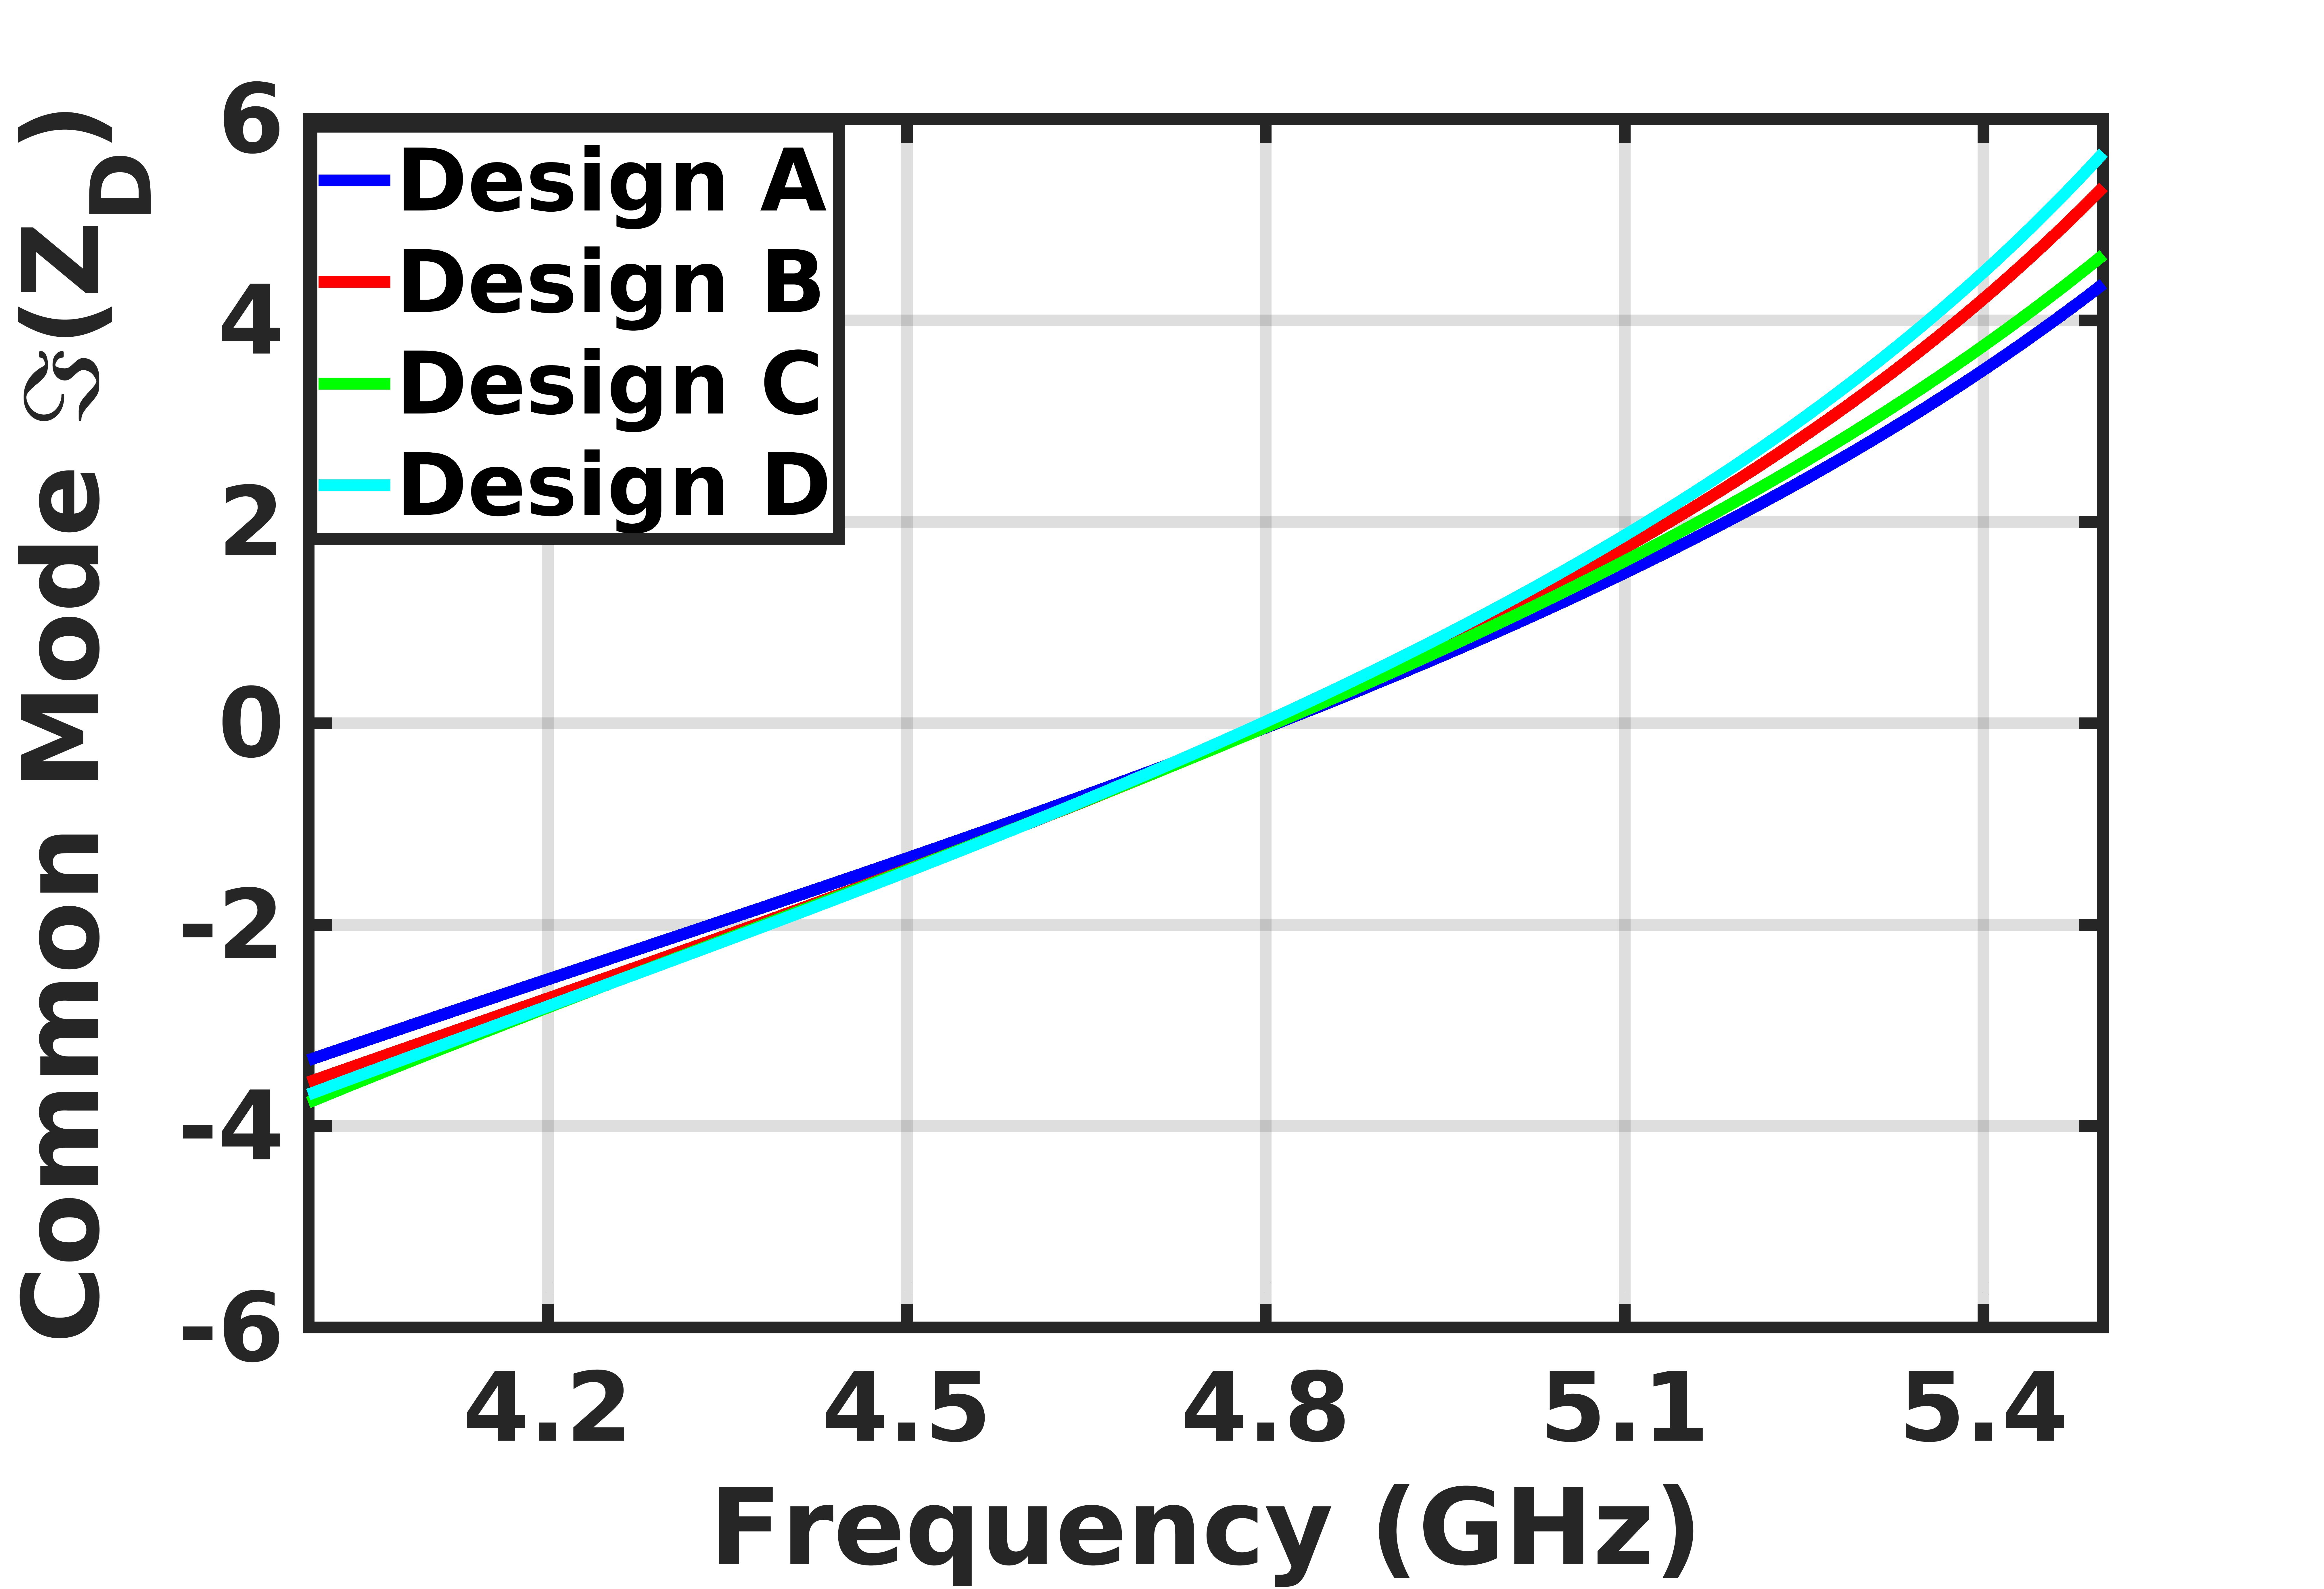
\includegraphics[width=1\textwidth]{Images/Output_Network_Comp/Comp_2H_imag.jpg}
\caption{}
\label{fig:Comp_2H_imag}
\end{subfigure}
\begin{subfigure}{0.24\textwidth}
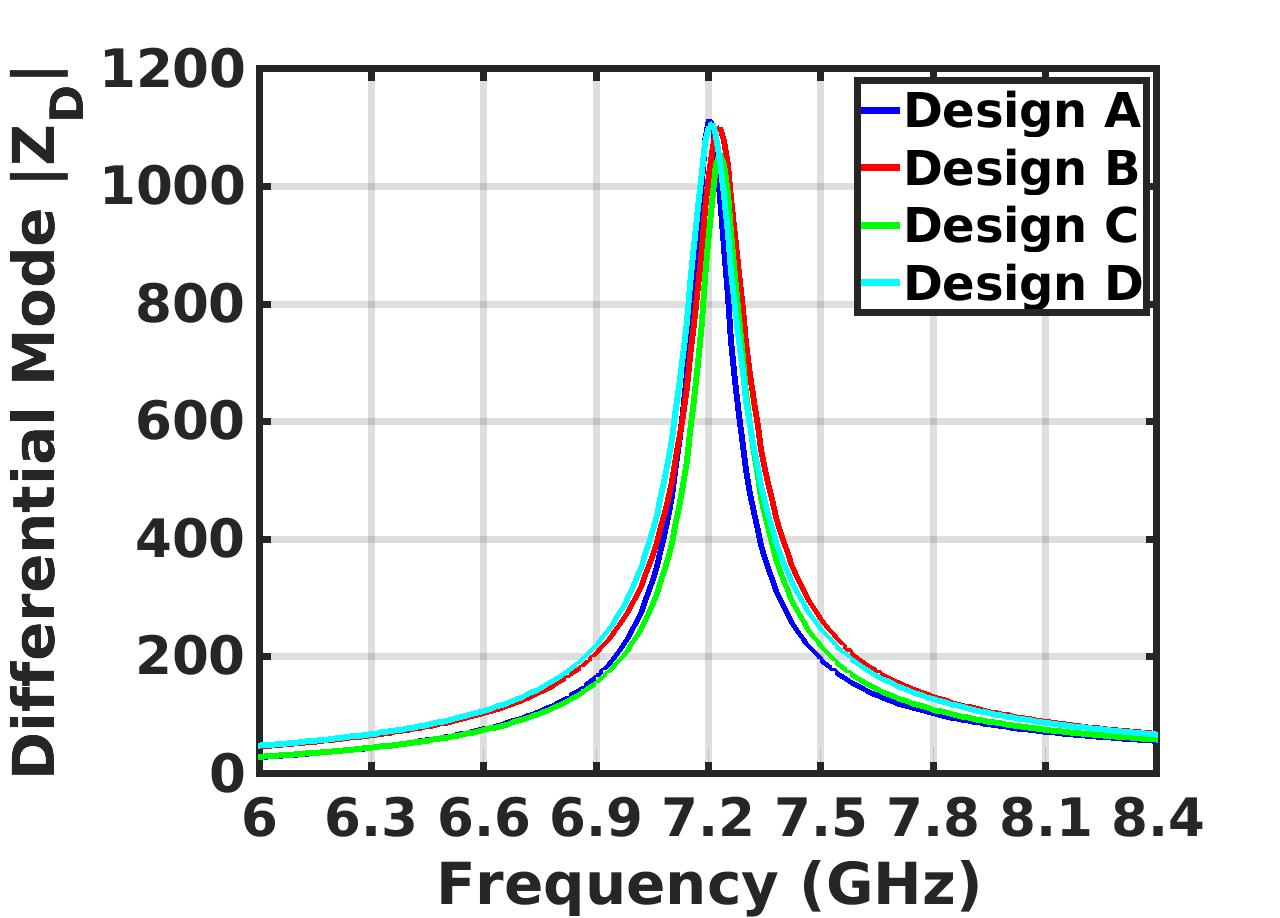
\includegraphics[width=1\textwidth]{Images/Output_Network_Comp/Comp_3H_Mag.jpg}
\caption{}
\label{fig:Comp_3H_Mag}
\end{subfigure}
\caption{(a) Impedance ($Z_D$) at $1^{st}$ harmonic, (b) Reactive part of $Z_D$ ($\Im(Z_D)$) at $2^{nd}$ harmonic, and (c) Magnitude of $Z_D$ ($|Z_D|$) at $3^{rd}$ harmonic.}
\label{fig:Comp_1H_2H_3H}
\vspace{-0.1in}
\end{figure}
The design A is tested with an ideal output stage (single transistor acting  as a current source when turned on) in ADS with lossless and lossy components
(Quality factor of \textit{7} for inductors, \textit{13} for transformer and \textit{100} for capacitors) 
to calculate peak $P_{OUT}$ and $\eta_D$ (Fig. \ref{fig:Comp_Pout_DE}). 
Further, Design A was implemented in TSMC 40 nm (Fig. \ref{fig:ON_X1}) and tested with the ideal output stage. The $km$ value was reduced to \textit{0.69} so as to achieve a layout friendly $L_P$ and $L_S$ and consequently, all the parameters were re-calculated as explained earlier. From Fig. \ref{fig:Comp_DE_loss_layout}, the proposed design in layout achieves a passive efficiency of \textit{52\%}.


\begin{figure}[!t]
\captionsetup{font=footnotesize}
\centering
\begin{subfigure}{0.24\textwidth}
\centering
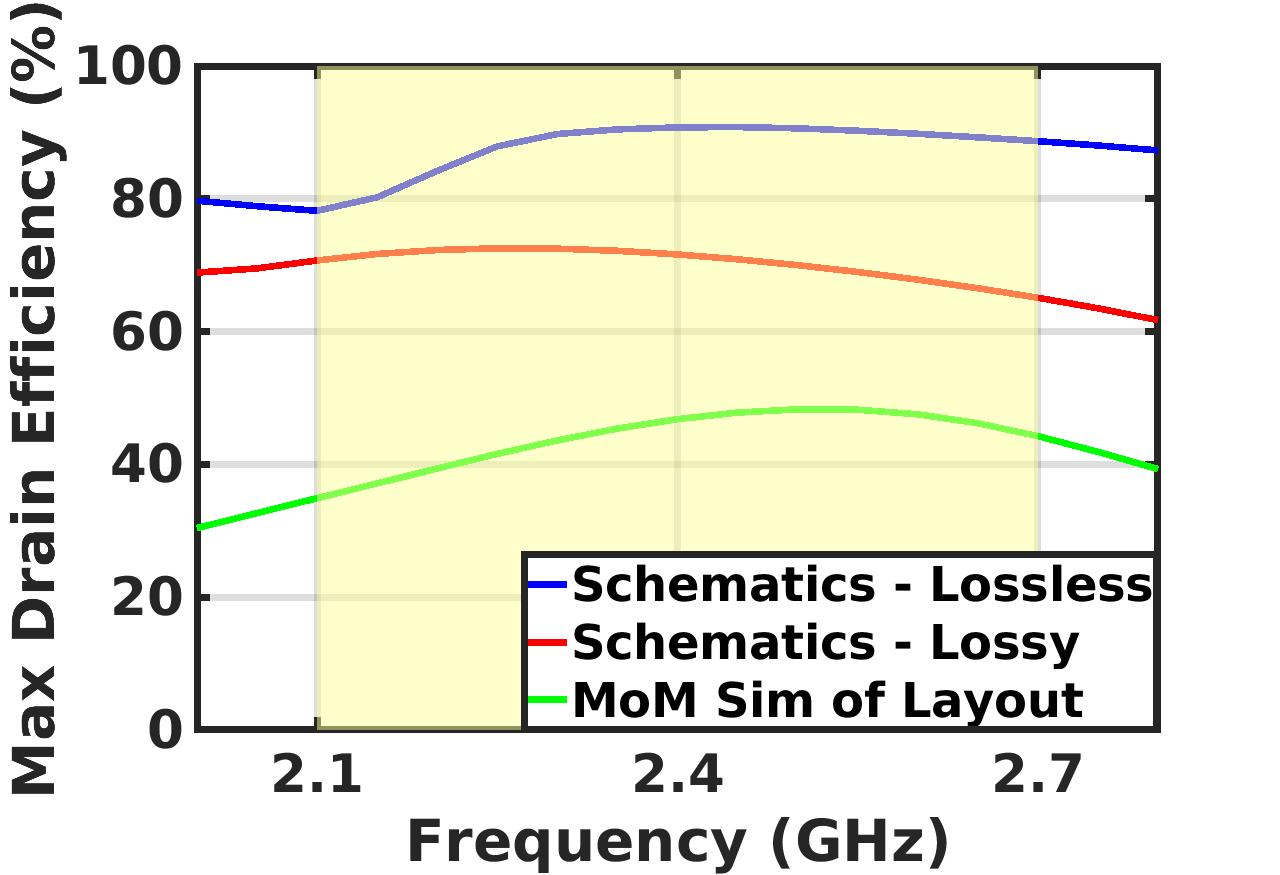
\includegraphics[width=1\textwidth]{Images/Output_Network_Comp/Comp_DE_loss_layout.jpg}
\caption{}
\label{fig:Comp_DE_loss_layout}
\end{subfigure}
\begin{subfigure}{0.24\textwidth}
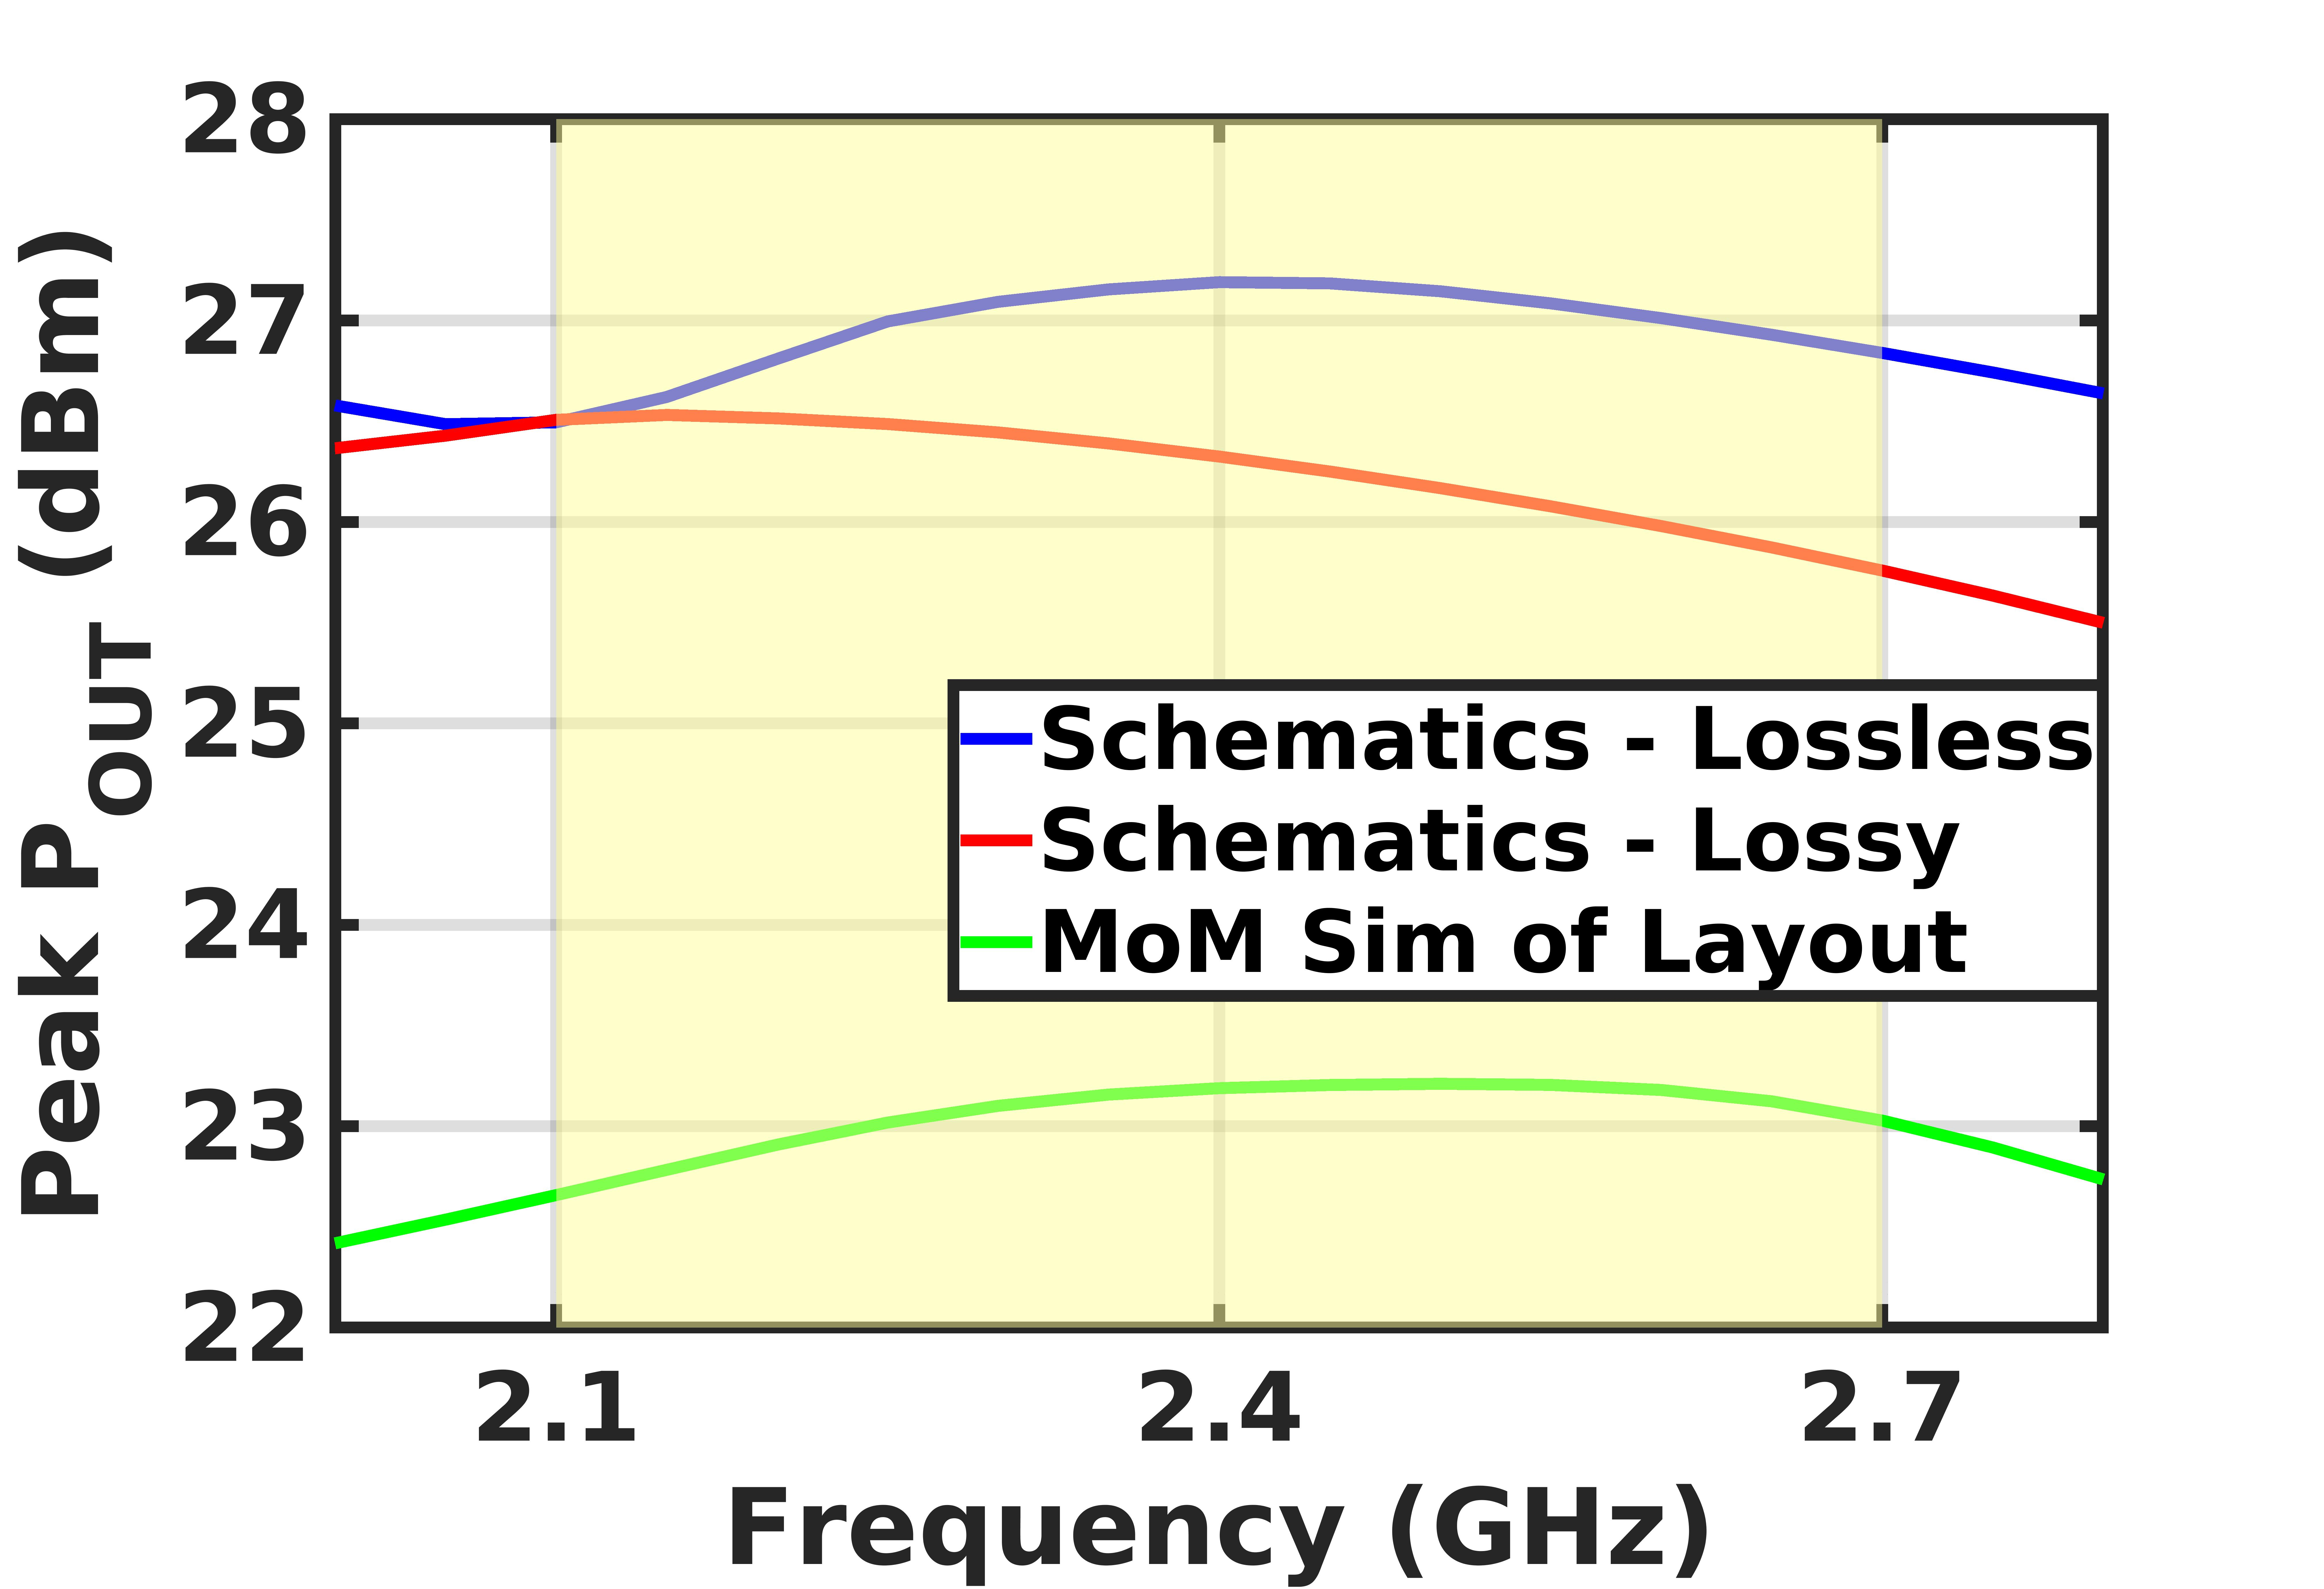
\includegraphics[width=1\textwidth]{Images/Output_Network_Comp/Comp_Pout_loss_layout.jpg}
\caption{}
\label{fig:Comp_Pout_loss_layout}
\end{subfigure}
\caption{(a) Maximum drain efficiency across frequency, and (b) Peak $P_{OUT}$ across frequency.}
\label{fig:Comp_Pout_DE}
\vspace{-0.1in}
\end{figure}

\begin{figure}[!t]
\centering
\captionsetup{font=footnotesize}
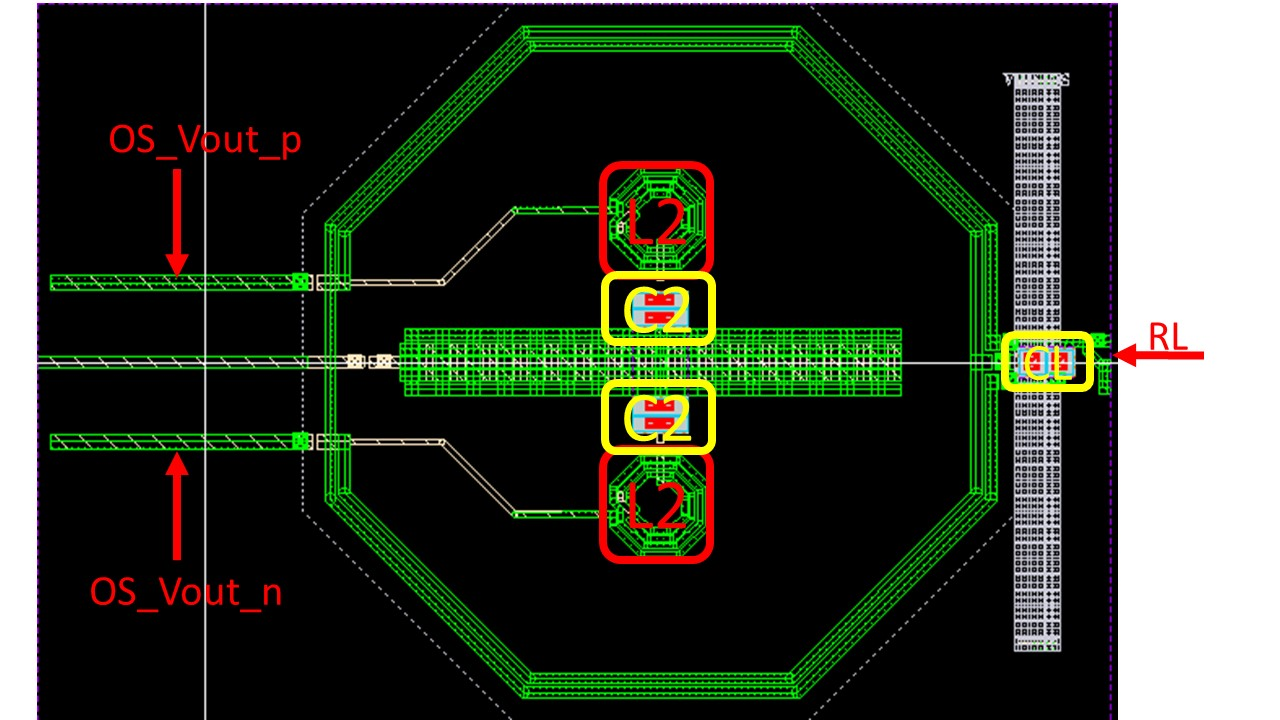
\includegraphics[width=0.93\linewidth]{Images/Output_Network_Comp/ON_X1.jpg}
\caption{Layout of the Design A (Balun, $L_2C_2$ and $C_L$).}
\label{fig:ON_X1}
\vspace{-0.25in}
\end{figure}

\section{Conclusion}
\label{section:Conclusion}
This paper presented CCF's wide operational bandwidth advantage over its class F companion. It detailed the primary requirement of the CCF PA output network, which is if the reactive part of $1^{st}$ harmonic decreases, then the reactive part of $2^{nd}$ harmonic should increase. Furthermore, the procedure to design the four different output networks for the \textit{2.1 -- 2.7 GHz} band was proposed and analyzed in detail.  Consequently, design A, with no RF choke and  including a 2$^{nd}$ harmonic trap, was chosen because it offers relatively constant output RF power in the desired frequency band with the least number of lumped components. Further, layout of design A was implemented in TSMC 40 nm and it achieved a passive efficiency of \textit{52\%}.

\bibliographystyle{IEEEtran}
\bibliography{disseration.bib}

\end{document}


